% !TEX root = ../my-thesis.tex
%
\chapter{Search for dark matter in association with a Higgs boson decaying to \(b\)-quarks}
\label{ch:monoH}

\section{Introduction}
\label{sec:monoH:introduction}
This chapter describes the search for dark matter in association with a Higgs boson \Ph decaying to \(b\)-quarks, referred to as \(\met + \Hbb\). The signature of the signal process is missing transverse momentum originating from the production of dark matter particles \(\chi\) and a pair of \btagged jets from the Higgs boson decay.
Searches for dark matter produced in association with Higgs bosons enable a direct investigation of the interaction of dark matter with the Higgs boson, as the initial state radiation of Higgs bosons is strongly Yukawa-suppressed.
The various decay modes of the Higgs boson allow for searches in final states with \bquarks, vector boson pairs, photons, and \Ptau leptons. This search focuses on the Higgs boson decaying to \bquarks, as it is the decay mode with the largest branching fraction \(\mathcal{B} = \SI{57}{\percent}\)~\cite{CERN2017}.

Searches for dark matter in the \(\met + \Hbb\) final state have been carried out by the ATLAS collaboration using \SI{20.3}{\per\femto\barn} \HepProcess{\Pp\Pp} collision data collected at a centre-of-mass energy \(\sqrt{s} = \SI{8}{\tera\electronvolt}\)~\cite{EXOT-2014-20} and using up to \SI{36.1}{\per\femto\barn} \HepProcess{\Pp\Pp} collision data collected at a centre-of-mass energy \(\sqrt{s} = \SI{13}{\tera\electronvolt}\)~\cite{EXOT-2015-23,EXOT-2016-25}. Similar searches have been carried out also by the CMS collaboration~\cite{CMS-EXO-16-012,CMS-EXO-16-050,CMS-EXO-18-011}.

This search is based on proton-proton collision data at a centre-of-mass energy of \SI{13}{\tera\electronvolt} recorded in the years 2015 -- 2017 with the ATLAS detector at the LHC, corresponding to an integrated luminosity of  \SI{79.8}{\per\femto\barn}.

Besides the more extensive data sample, the search benefits from two novel reconstruction techniques, which result in enhanced sensitivity to previous results. The improved identification of \bjets which is based on track jets with a variable radius parameter enhances the reconstruction efficiency of highly boosted Higgs boson candidates. The use of an object-based \met significance, which fully accounts for the resolutions and correlations of the objects entering the \met reconstruction, enables the efficient suppression of processes with fake \met.
The results of this search have been presented in Ref.~\cite{ATLAS-CONF-2018-039}.

\Cref{sec:monoH:physics} introduces the signal and background processes in the \(\met + \Hbb\) search. The analysis strategy is outlined in \Cref{sec:monoH:analysis}. The object and event selection, including the definition of the signal region, is described in \Cref{sec:monoH:selection}, whereas the background estimation strategy and the definitions of the control regions are described in \Cref{sec:monoH:backgrounds}.
The systematic uncertainties taken into account in the statistical model are described in \Cref{sec:monoH:systematics}, while the statistical model itself is provided in \Cref{sec:monoH:model}. Finally, the observed results are presented and discussed in \Cref{sec:monoH:results}. A conclusion is given in \Cref{sec:monoH:conclusion}.


\section{Signal and background processes}
\label{sec:monoH:physics}
The analysis investigates dark matter production in the framework of the \zhdm simplified model, which is described in \Cref{sec:monoH:physics:zhdm}. The background processes are described in \Cref{sec:monoH:physics:backgrounds}.  The simulated signal and background samples are summarised in \Cref{sec:monoH:physics:mcsamples}.

\subsection{\zhdm simplified model}
\label{sec:monoH:physics:zhdm}
The \zhdm simplified model, a type-II two-Higgs-doublet model (2HDM) with an additional \(\text{U}(1)_{\PZprime}\) gauge symmetry (c.f. \Cref{sec:dm:models:zp2hdm}), is considered for the optimisation of the search and the interpretation of its results.
The process yielding the signature of \(\met + \Hbb\) is illustrated in \Cref{fig:monoH:physics:zhdm:graph}.

\begin{figure}[hbtp]
  \centering
  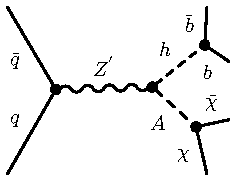
\includegraphics[width=0.4\textwidth]{figures/monoH/mono_h_zprime.pdf}
  \caption{Production of dark matter particles \(\chi\) and a Higgs boson \Ph through a new \PZprime mediator coupled to the CP-odd Higgs boson \PA, where the latter decays primarily to \(\chi \overline{\chi}\).}
  \label{fig:monoH:physics:zhdm:graph}
\end{figure}

A \PZprime vector boson is produced in \HepProcess{\Pp\Pp} collisions and decays into the neutral Higgs boson \Ph, which is identified with the SM Higgs boson in the alignment limit, and the CP-odd Higgs boson \PA. The latter decays into dark matter particles, which give rise to missing transverse momentum \met.
A characteristic feature of the model is that for heavy \PZprime boson masses, the predicted \met spectra are much harder than for other models describing the \(\met + \Hbb\) signature~\cite{Abercrombie2019}.

The relevant model parameters and their chosen values are listed in \Cref{tab:monoH:physics:zhdm:parameters}. These parameters include the masses of the involved particles \mA, \mZp, \mchi, and the gauge coupling of the \PZprime boson to quarks \gZp. The dark matter particle mass \mchi has negligible impact on the results for \(2 \mchi < \mA\) and is set to \SI{100}{\giga\electronvolt}. The value of the ratio of the vacuum expectation values (VEV) of the two Higgs fields is chosen as \num{1.0}, thereby satisfying perturbativity requirements due to the top-quark Yukawa coupling~\cite{Berlin2014}. As the alignment limit \(\alpha = \beta - \pi / 2\) is considered, the lightest neutral scalar boson is identified with the SM Higgs boson with \(\mHiggs = \SI{125}{\giga\electronvolt}\). The masses of the heavy scalar Higgs boson and of the charged Higgs bosons are set to \(\mHiggsHeavy = \mHiggsCharged = \SI{300}{\giga\electronvolt}\).

The \zhdm model is used as a benchmark to probe the \(\met + \Hbb\) signature in a generic way. In particular, the discriminating variables deliberately do not exploit the characteristic features of the resonant production of \HepProcess{\Ph \chi \overline{\chi}}, such as the Jacobian peak in the Higgs boson's \pt distribution with an endpoint at
\begin{align}
    \pt^{\Ph, \text{max.}} = \frac{\sqrt{(m^{2}_{\PZprime} - m^{2}_{\Ph} - m^{2}_{A})^2 - 4 m^{2}_{\Ph} m^{2}_{A}}}{2 m_{\PZprime}}.
\end{align}
Although the chosen value of \(\gq = 0.8\), which was initially recommended by the LHC DM WG~\cite{Abercrombie2019}, is already excluded by dijet searches~\cite{EXOT-2017-32}, it is adopted to allow for the direct performance comparison to the results of the previous iteration~\cite{EXOT-2016-25}.
The branching fraction of the decay \HepProcess{\PA \to \chi \overline{\chi}} is assumed to be \SI{100}{\percent} for the interpretation of the results.

The results of the search are interpreted for a scan over the two-dimensional \mZp-\mA plane for fixed choices of the other model parameters. The scan extends over the range \SIrange{400}{3000}{\giga\electronvolt} in \mZp and \SIrange{300}{800}{\giga\electronvolt} in \mA.

\begin{table}[htbp]
\caption{Parameters of the \zhdm simplified model in the \(\met + \Hbb\) search.}
\label{tab:monoH:physics:zhdm:parameters}
\centering
\begin{tabular}{l l r}
\toprule
Parameter & Description & Chosen value \\
\midrule
\mHiggs & light CP-event Higgs boson mass & \SI{125}{\giga\electronvolt} \\
\mZp & \PZprime boson mass & free \\
\mA & CP-odd Higgs boson mass & free \\
\mchi & dark matter particle mass & \SI{100}{\giga\electronvolt}\\
\mHiggsHeavy & heavy Higgs boson mass & \SI{300}{\giga\electronvolt} \\
\mHiggsCharged & charged Higgs boson mass & \SI{300}{\giga\electronvolt} \\
\gZp & \PZprime gauge coupling to quarks & 0.8 \\
\(\tan{\beta}\) & ratio of Higgs VEV & 1  \\
\(\alpha\) & mixing of \Ph and \PH & \(-\pi / 4\)\\
\bottomrule
\end{tabular}
\end{table}


\subsection{Background processes}
\label{sec:monoH:physics:backgrounds}
The dominant background processes with the signature of two \bjets and substantial \met are \ttbar production (\SI{50}{\percent} background contribution), \zjets production (\SI{33}{\percent} background contribution), and \wjets production (\SI{15}{\percent} background contribution).

Sub-dominant background processes include \HepProcess{\PW \PW}, \HepProcess{\PW \PZ}, and \HepProcess{\PZ \PZ} diboson production, single top quark production, SM \VHbb production, and multijet events.

The dominant background processes are estimated using simulated samples, whose normalisation is constrained by control region data. The smaller background processes are estimated purely by simulation. Based on a data-driven estimate, it will be shown in \Cref{sec:monoH:backgrounds:multijet} that the multijet background is negligible.


\subsection{Simulated Monte Carlo samples}
\label{sec:monoH:physics:mcsamples}
The signal and background processes with the MC event generators, parton shower models and PDF sets used for their description are summarised in \Cref{tab:monoH:physics:mcsamples:generators}. Detailed descriptions of the background samples are provided in \Cref{sec:common:data:mc}.

The signal process in the \zhdm simplified model is simulated on a grid of \num{53} mass points defined by the mediator mass \mZp and the CP-odd Higgs boson mass \mA.
The mass of the \PZprime boson is scanned in the range \SIrange{400}{3000}{\giga\electronvolt} in steps of \SI{200}{\giga\electronvolt} and the mass of the CP-odd Higgs boson \PA is scanned in the range \SIrange{300}{800}{\giga\electronvolt} in \SI{100}{\giga\electronvolt} steps for the relevant regions of phase space.

The simulated events are generated at leading-order (\LO) accuracy in QCD with the \MGMCatNLOV{2.2.3} event generator~\cite{Alwall:2014hca} interfaced to the \PYTHIAV{8.186}~\cite{Sjostrand:2014zea} parton shower and hadronisation model, using the \textsc{NNPDF30} PDF set~\cite{Ball2015} and the \AFourteen set of tuned parameters~\cite{ATL-PHYS-PUB-2014-021}.

\begin{table}[htbp]
\caption{List of the signal and background processes with the MC event generators, sets of PDFs and tunes used for their description in the \(\met + \Hbb\) search.}
\label{tab:monoH:physics:mcsamples:generators}
\centering
\resizebox{1.\textwidth}{!}{%
\begin{tabular}{l l l}
\toprule
Process & Generator & PDF / parton shower tune \\
\midrule
\textbf{Signal}  & & \\
\zhdm            & \MGMCatNLOV{2.2.3} & \textsc{NNPDF30LO} / \AFourteen \\
simplified model & + \PYTHIAV{8.212} & \\
\midrule
\textbf{Top quark}   & & \\
\ttbar               & \POWHEGBOXV{2} + \PYTHIAV{8.230} & \textsc{NNPDF30NLO} / \AFourteen \\
\Pqt (\(s\)-channel) & \POWHEGBOXV{2} + \PYTHIAV{8.230} & \textsc{NNPDF30NLO} / \AFourteen \\
\Pqt (\(t\)-channel) & \POWHEGBOXV{2} + \PYTHIAV{8.230} & \textsc{NNPDF30NLO} / \AFourteen \\
\Pqt (\(\PW t\))     & \POWHEGBOXV{2} + \PYTHIAV{8.230} & \textsc{NNPDF30NLO} / \AFourteen \\
\midrule
\textbf{\(V\) + jets} & & \\
\Wjets & \SHERPAV{2.2.1} & \textsc{NNPDF30NNLO} / \SHERPA-tune \\
\Zjets & \SHERPAV{2.2.1} & \textsc{NNPDF30NNLO} / \SHERPA-tune \\
\midrule
\textbf{Diboson}    & & \\
\HepProcess{\PW\PW} & \SHERPAV{2.2.1}                  & \textsc{NNPDF30NLO} / \SHERPA-tune \\
\HepProcess{\PW\PZ} & \SHERPAV{2.2.1}                  & \textsc{NNPDF30NLO} / \SHERPA-tune \\
\HepProcess{\PZ\PZ} & \SHERPAV{2.2.1}                  & \textsc{NNPDF30NLO} / \SHERPA-tune \\
\VHbb               & \POWHEGBOXV{2} + \PYTHIAV{8.212} & \textsc{NNPDF30NLO} / \AZNLO \\
\bottomrule
\end{tabular}%
}
\end{table}


\section{Analysis strategy}
\label{sec:monoH:analysis}
The signature of dark matter particle production in association with a Higgs boson is provided by missing transverse momentum \met recoiling against a system of two \bjets resulting from the Higgs boson decay \HepProcess{\Ph \to \Pqb \Paqb}.

The signal region (SR) is defined by the requirement of substantial \met and a Higgs boson candidate.
In events with a moderately boosted Higgs boson, the Higgs boson candidate can be reconstructed using two well-separated \btagged small-radius jets (resolved event topology). This approach fails for events with a highly boosted Higgs boson, as the smaller separation of the jets due to the Higgs boson's Lorentz boost does not allow for their individual reconstruction. Therefore, it is advantageous to reconstruct the Higgs boson candidate using a single large-radius jet, which is supplemented with sub-jets based on ID tracks to identify the two \bquarks.

Consequently, the signal region selection considers both the resolved and the merged event topologies. The distinction between these two categories is provided by \met, which is strongly correlated with the boost of the Higgs boson candidate. The boundary at \SI{500}{\giga\electronvolt} is chosen to enhance the sensitivity of the search in the merged category, since for large \met the SM backgrounds are strongly suppressed. The resolved category provides complementary sensitivity to signals with a moderate boost.

The two event topologies are similar to those considered in the \(\met + \Vqq\) search, which are illustrated in \Cref{fig:monoV:physics:topologies}.

Further requirements on kinematic properties and the event topology reduce the contribution of background processes. The main discriminating variable in the statistical analysis is the invariant mass of the Higgs boson candidate. Additional information is provided by the coarsely binned \met distribution. The resolved selection is defined for three \met bins, which extend from \SIrange{150}{200}{\giga\electronvolt}, \SIrange{200}{350}{\giga\electronvolt}, and \SIrange{350}{500}{\giga\electronvolt}. The merged selection is defined for events with more than \SI{500}{\giga\electronvolt}.

The control regions (CRs) are defined by the lepton multiplicity in the event (c.f. \Cref{sec:common:analysis}) and cover a similar phase-space as the SR. As SR and CRs have different requirements on the lepton multiplicity, they do not overlap. The SR selection vetoes events containing electrons or muons. The control regions, in turn, require the presence of either one muon (1 muon CR) or two electrons or muons (2 lepton CR).
Instead of \met, the 1 muon selection employs the \metnomu variable, which is constructed by adding the muon momentum vector to \met. Similarly, the 2 muon selection uses the transverse momentum of the dilepton system \ptll. These variables emulate the way how the background processes can enter the SR.

The SR and CRs considered in the analysis are
\begin{itemize}
	\item 0 lepton SR with no electrons and no muons, requiring two \bjets, partitioned in three \met bins in the resolved category and one in the merged category,
	\item 1 muon CR with one muon and no electrons, requiring two \bjets, partitioned in three \metnomu bins in the resolved category and one in the merged category,
	\item 2 lepton CR with two same-flavour leptons, requiring two \bjets, partitioned in three \ptll bins in the resolved category and one in the merged category.
\end{itemize}

A graphical overview of all regions and categories considered in the analysis with their relative background composition is given in \Cref{fig:monoH:analysis:overview}.
\begin{figure}[htbp]
	\centering
	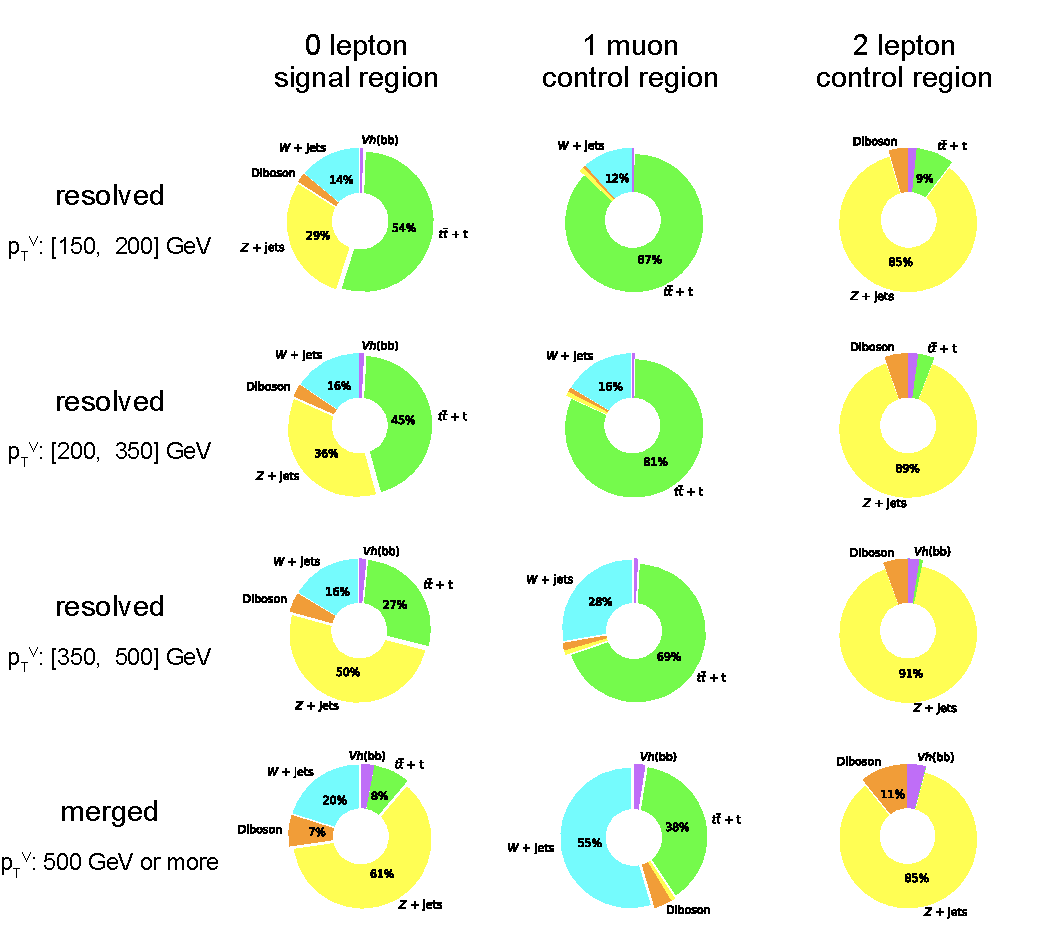
\includegraphics[width=1.\textwidth]{figures/monoH/monoHoverview.pdf}
	\caption{Overview of all regions and \ptv bins considered in the \(\met + \Hbb\) search with their relative background composition, where \ptv denotes \met in the signal region, \metnomu in the 1 muon control region, and \ptll in the 2 lepton control region, respectively. Each region consists of three resolved event-topology \ptv bins and the merged event-topology \ptv bin.}
	\label{fig:monoH:analysis:overview}
\end{figure}


\section{Object and event selection}
\label{sec:monoH:selection}
The event selection requirements for events considered in the SR are outlined below. The specific choices for physics object definitions are summarised in \Cref{sec:monoH:selection:objects}.
The common baseline selection used in SR and CRs is described in \Cref{sec:monoH:selection:baseline}, while the SR event selection is described in \Cref{sec:monoH:selection:sr}.

\subsection{Object selection}
\label{sec:monoH:selection:objects}
The physical compound objects used in the \(\met + \Hbb\) search are based on the object definitions, which are introduced in \Cref{sec:common:objects}.

Two novel object definitions are exploited --- the variable radius track jets, which extend the sensitivity of the search in case of large boosts of the Higgs boson candidate, and an object-based \met significance, which serves the rejection of background processes with fake \met.

Central jets and forward jets are used to define selection requirements on the event topology, which suppress background processes. The \bjets are identified by \btagging algorithms, using the MV2 discriminant with a fixed-cut working point corresponding to \SI{77}{\percent} \btagging efficiency.
The Higgs candidate reconstruction is based on the two most energetic \bjets in the resolved category and on the most energetic large-radius jet in the merged category.

The identification of the large-radius jet flavour content is based on track jets associated with the large-radius jet via ghost-matching. The track jets allow for maintaining high double \btagging efficiency in the merged event topology. However, for substantially large Higgs boson momenta, even the track jets can overlap if they are reconstructed with a fixed radius parameter. The problem of track jet merging is overcome by the use of variable-radius (VR) track jets, as illustrated in \Cref{fig:monoH:selection:objects:vrtrackjets-efficiency}.

\begin{figure}[h]
  \centering
  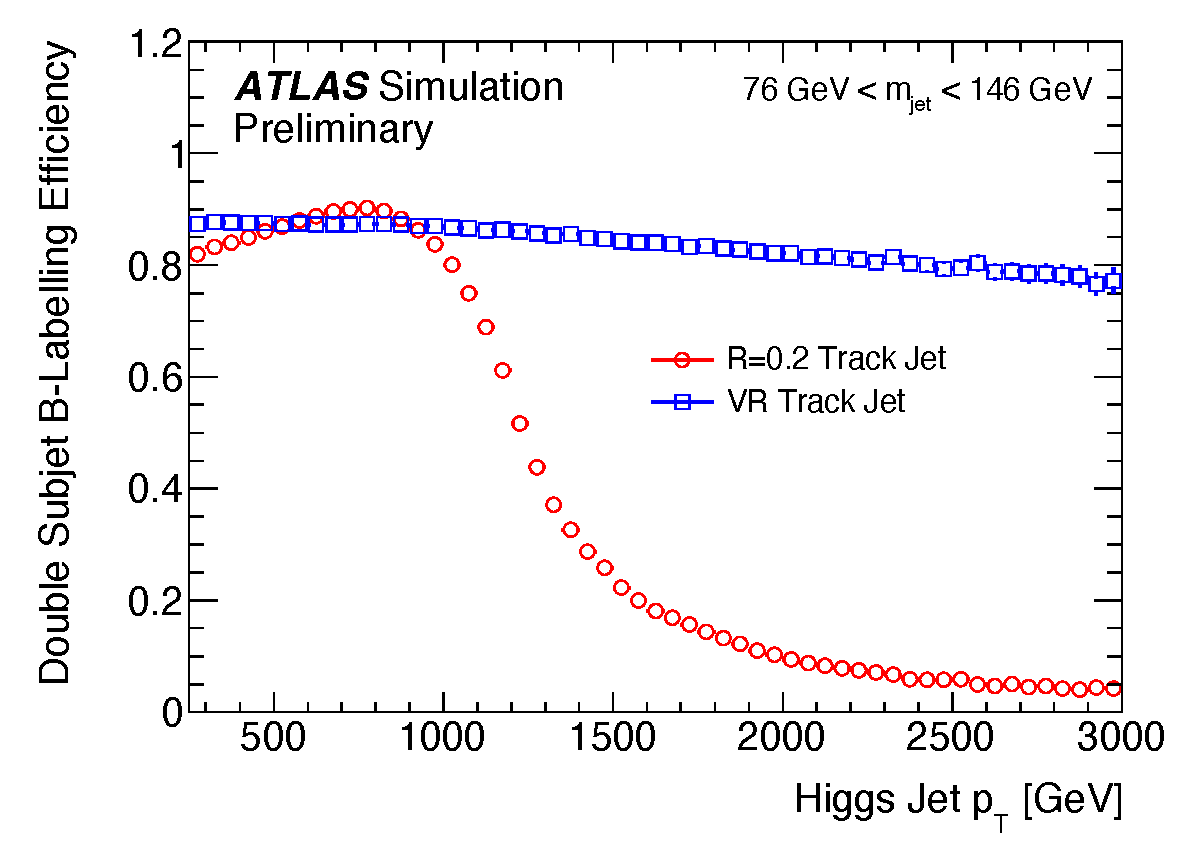
\includegraphics[width=0.95\textwidth]{figures/monoH/vrtrackjets2.pdf}
  \caption{The efficiency for a large-radius jet from a \Htobb decay (referred to as Higgs jet) to have its two associated sub-jets with largest transverse momentum matched to truth \PB-hadrons in dependence of its \pt. The error bars include statistical uncertainties only. Figure modified from Ref.~\cite{ATL-PHYS-PUB-2017-010}.}
  \label{fig:monoH:selection:objects:vrtrackjets-efficiency}
\end{figure}

The use of the VR track jets allows maintaining a high double \btagging efficiency over a broad Higgs boson momentum range, which overall is superior to conventional FR track jets.
Therefore, the identification of \bjets in the merged category is based on VR track jets.

The charged lepton definitions are similar to those used in the \(\met + \HepProcess{V(\Pq\Pq)}\) search (c.f. \Cref{sec:monoV:selection:objects}), except for the \(E_{\text{T}} > \SI{27}{\giga\electronvolt}\) requirement in the signal electron candidate definition due to the increased single electron trigger threshold in 2017 data-taking. Baseline electron and muon candidates are used for the definition of lepton vetoes in the SR, as the baseline definition aims at providing a high reconstruction efficiency. Signal electron and muon candidates are used to select electron or muon pairs for the 2 lepton CR, where a high purity selection is desired. Tight signal muons are used to select muons in the 1 muon CR.
In addition, baseline tau lepton candidates are used to define vetoes on tau leptons in the event selection.

The missing transverse momentum \met is reconstructed from the calibrated physics objects in the event and the track-based soft term (TST) using the \textsc{Loose} working point.
Closely related definitions are employed in the CRs to accommodate how background processes are contributing to the SR. In the 1 muon CR, the \metnomu variable is used, which is reconstructed by excluding muons from the \met  calculation, thereby adding the muon momentum vector to \met. Similarly, in the 2 lepton CR, the transverse momentum of the dilepton system \ptll is used.

The object-based \met significance \(\mathcal{S}\) is used to separate events in which the reconstructed missing transverse momentum \met is genuinely coming from dark matter particles or neutrinos from events with fake \met caused by resolution effects.

\Cref{fig:monoH:selection:objects:metsignificance} illustrates the performance of the object-based \met significance in comparison to an event-based definition of \met significance \(\met / \sqrt{\sum \met}\) and \met itself in the \(\met + \Hbb\) search. The object-based \met significance definition is clearly superior, as a requirement of \(\mathcal{S} > 16\) can reject over \SI{95}{\percent} of background processes with fake \met while retaining a signal efficiency over \SI{90}{\percent}. In contrast, the event-based \met significance achieves similar background rejection with a signal efficiency of \SI{80}{\percent}, while the use of \met decreases the signal efficiency to \SI{30}{\percent}.

\begin{figure}[htbp]
  \centering
  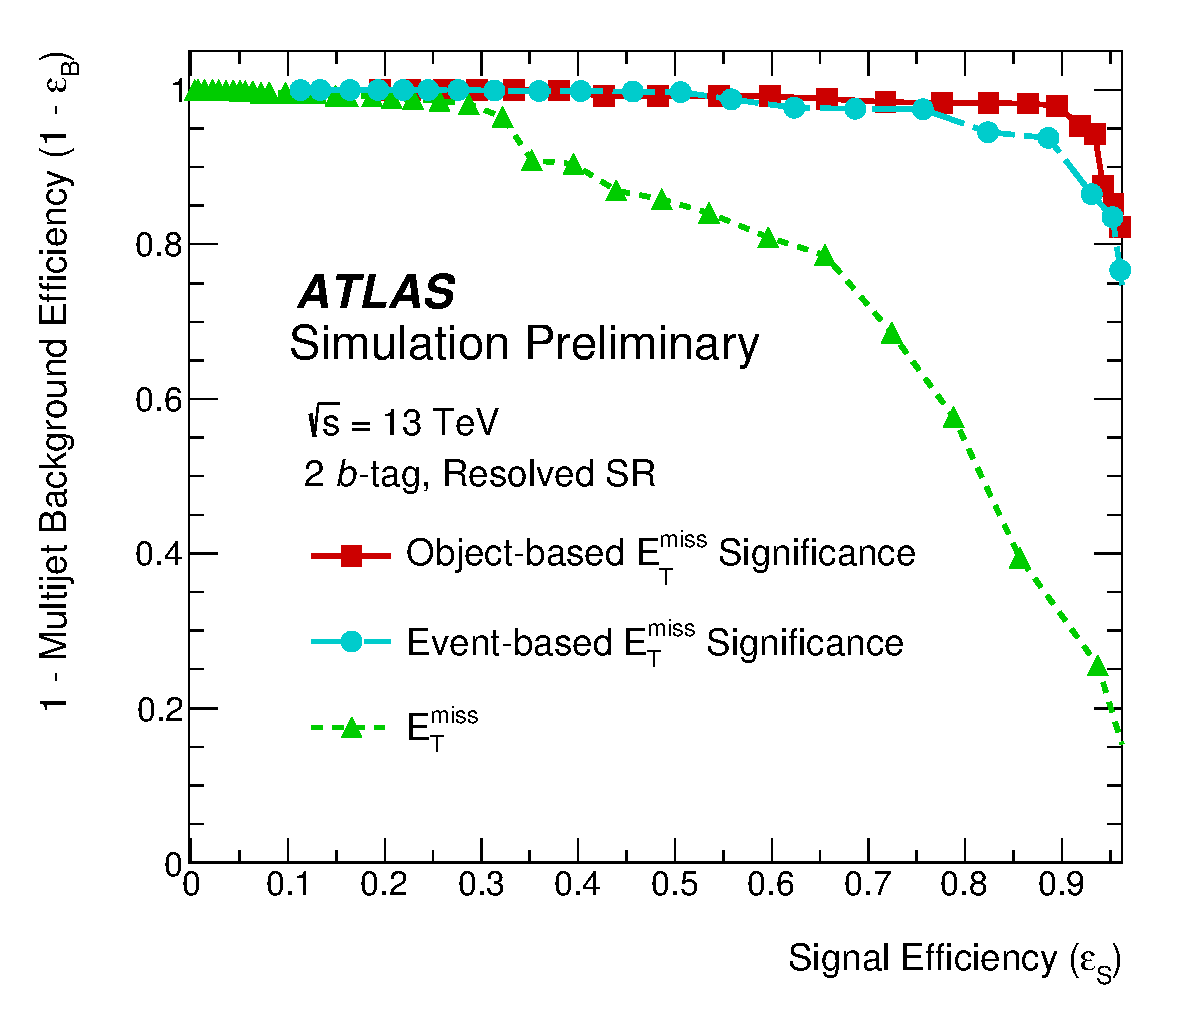
\includegraphics[width=1.\textwidth]{figures/monoH/metsignificance.pdf}
  \caption{Performance of the \met significance (line with square markers) in terms of the signal efficiency and multijet background rejection in the \(\met + \Hbb\) search, compared to an event-based \met significance definition  \(\met / \sqrt{\sum \met}\) (dashed line with circular markers), and on \met itself (densely-dashed line with triangular markers). The signal efficiency is estimated with a \zhdm signal sample with \(\mZp = \SI{400}{\giga\electronvolt}\) and \(\mA = \SI{300}{\giga\electronvolt}\), which has a very soft \met distribution, whereas the background rejection is estimated with a sample of simulated dijet events. The events used for the comparison are selected by the \(\met + \Hbb\) baseline selection requirements, including a requirement on the angular separation between the \met vector and the three jets with highest \pt.}
  \label{fig:monoH:selection:objects:metsignificance}
\end{figure}

Potential ambiguities in the reconstruction, such as reconstructed objects matching multiple object hypotheses, must be resolved by an overlap removal procedure. The overlap removal procedure applies six stages in the order listed as follows.
\begin{enumerate}
  \item Electron-electron overlap removal. If an event contains two reconstructed electrons sharing a track, the electron candidate with lower \pt is removed from the event.
  \item Tau-electron and tau-muon overlap removal. If an event contains a reconstructed tau lepton within the distance \(\Delta R < 0.2\) of any reconstructed electron or muon, the tau candidate is removed from the event.
  \item Electron-muon overlap removal. If an event contains a reconstructed electron and a reconstructed muon sharing the same track, the electron candidate is removed from the event.
  \item Electron-jet overlap removal. All jets within the distance\footnote{The distance measure employed for the overlap removal procedure is based on the rapidity distance \(\Delta y\) instead of the pseudorapidity distance \(\Delta \eta\).} \(\Delta R = \sqrt{\Delta y^2 + \Delta \varphi^2} < 0.2\) of electrons surviving the previous stage of the overlap removal procedure are removed from the event. Then, all reconstructed electrons of transverse energy \(E_{\text{T}}\) within the distance \(\min\{0.4, 0.04 + \SI{10}{\giga\electronvolt} / E_{\text{T}}\}\) of jets are removed from the event.
  \item Muon-jet overlap removal. All jets within the distance \(\Delta R < 0.2\) of any reconstructed muon are removed, if they either have fewer than three associated tracks or if the muon \pt is greater than \(\max\{0.5 \, \pt^{\text{jet}}, 0.7 \sum_{i} \pt^{\text{track, i}}\}\), where \(\pt^{\text{track}}\) denotes the transverse momentum of tracks associated to the jet. Then, all reconstructed muons of transverse momentum \pt within the distance \(\min\{0.4, 0.04 + \SI{10}{\giga\electronvolt} / \pt\}\) of jets are removed from the event.
  \item Overlap removal between large-radius-jets and electrons. If an event contains a large-radius jet within the distance \(\Delta R < 0.1\) of an electron, the large-radius jet is removed from the event.
\end{enumerate}


\subsection{Baseline selection}
\label{sec:monoH:selection:baseline}
The SR and CR definition is based on a common baseline selection and common requirements to suppress the multijet background. These selection requirements are almost identical to the those used in the \(\met + \HepProcess{V(\Pq\Pq)}\) search, which are presented in \Cref{sec:monoV:selection:baseline} and \Cref{sec:monoV:selection:antiqcd}, respectively. There are three exceptions, which concern the jet cleaning requirement in the baseline selection and the definition of the multijet-suppression requirements.
\begin{itemize}
 	\item The jet cleaning selection requirement is solely based on the \textsc{BadLoose} definition. No additional requirement based on the \textsc{Tight} jet cleaning definition is made.
 	\item Only the \(\min \Delta \varphi(\text{jets}_{1,2,3}, \met) > \SI{20}{\degree}\) and the \(\Delta \varphi(\met, \mpt) < \SI{90}{\degree}\) multijet-suppression requirements are applied. The requirement that the azimuthal distance between \met and the boson candidate has to exceed \SI{120}{\degree} and the requirement on \(\mpt > \SI{30}{\giga\electronvolt}\) are no longer part of the common baseline selection.
 	\item These multijet-suppression requirements are only applied in the SR and in the 1 muon CR selection but not in the 2 lepton CR. The 2 lepton CR selection sufficiently suppresses potential contamination through multijet events and would suffer from large statistical uncertainty if the multijet-suppression requirements were applied.
 \end{itemize}

The baseline selection requirements are summarised in \Cref{tab:monoH:selection:baseline:summary}.
\begin{table}[hbtp]
\caption{List of the baseline event selection requirements employed in the \(\met + \Hbb\) search.}
\label{tab:monoH:selection:baseline:summary}
\centering
\resizebox{1.\textwidth}{!}{%
\begin{tabular}{l lll}
\toprule
Baseline selection & 0 lepton SR & 1 muon CR & 2 lepton CR \\
\midrule
Data quality & \multicolumn{3}{c}{basic requirements vetoing corrupted data or incomplete events} \\
Vertex reconstruction & \multicolumn{3}{c}{primary vertex with at least two associated tracks} \\
Jet cleaning & \multicolumn{3}{c}{veto on events containing jets flagged as \textsc{BadLoose} jets} \\
Trigger & \met trigger & \met trigger & single lepton trigger \\
\midrule
\multirow{3}{*}{Multijet suppression} & \(\min \Delta \varphi(\text{jets}_{1,2,3}, \met) > \SI{20}{\degree}\) & \(\min \Delta \varphi(\text{jets}_{1,2,3}, \metnomu) > \SI{20}{\degree}\) & no \\
& \(\Delta \varphi(\met, \mpt) < \SI{90}{\degree}\) & \(\Delta \varphi(\metnomu, \mptnomu) < \SI{90}{\degree}\) & no \\
\bottomrule
\end{tabular}%
}
\end{table}

\subsection{Signal region selection}
\label{sec:monoH:selection:sr}
As the signature sought by the \(\met + \Hbb\) search does not involve leptons, a veto on events containing baseline muons or baseline electrons is employed in the SR event selection.

Following the baseline selection requirements, events are separated into the resolved and merged categories using a single selection requirement on \met.

The \textbf{resolved category} event selection is optimised for events with a moderate amount of missing transverse momentum \(\SI{150}{\giga\electronvolt} < \met < \SI{500}{\giga\electronvolt}\) and a Higgs boson candidate, whose decay products can be resolved by two \btagged small-radius jets. The jets used for the Higgs boson candidate reconstruction are the two \bjets with highest \pt in the event and are referred to as \(j_1\) and \(j_2\). The invariant mass of the dijet system composed out of these jets, which is referred to as \(m_{jj}\), provides strong discrimination between signal and background processes, as Higgs boson candidates exhibit a characteristic mass peak at the Higgs boson mass.

The remaining selection requirements are similar to those of the \(\met + \Vqq\) search, as a similar event topology is targeted. In events with exactly two central jets, their scalar transverse momentum sum is required to be larger than \SI{120}{\giga\electronvolt}, whereas in events with three or more central jets, instead the scalar transverse momentum sum of the three central jets with highest \pt is required to be larger than \SI{150}{\giga\electronvolt}. At least one of the jets used to reconstruct the Higgs boson candidate is required to have a transverse momentum greater than \SI{45}{\giga\electronvolt}.

In addition to the multijet-suppression requirements outlined in \Cref{sec:monoH:selection:baseline}, four requirements are explicitly introduced for the resolved category to reduce the contribution of multijet processes.
The jets used for the Higgs boson candidate reconstruction often are in a back-to-back topology for multijet events, whereas they are in close proximity for the signal process. Therefore, the requirements on the separation of the Higgs boson candidate jets \(\Delta\varphi(j_{1},j_{2}) < \SI{140}{\degree}\) and \(\Delta R(j_{1},j_{2}) < 1.8\) are introduced.
In signal-like events the missing transverse momentum is expected to be in a back-to-back topology with the Higgs boson candidate, motivating the requirement on the azimuthal distance between \met and the Higgs boson candidate \(\Delta\varphi(\met , \Ph) > \SI{120}{\degree}\). The specific values used in these requirements are chosen by examining distributions of these observables for excesses of data over the simulated non-multijet backgrounds, which are attributed to multijet backgrounds. These studies were validated with simulated multijet events.
Finally, a requirement based on the object-based \met significance \(\mathcal{S} > 16\) suppresses the remaining contributions of backgrounds with fake \met (c.f.~\Cref{sec:monoH:selection:objects}).

Although the \ttbar, \tWb background processes with \PW bosons decaying to electrons and muons are suppressed by the lepton vetoes, those with hadronically decaying tau leptons can still pass the event selection.
Therefore, an additional veto on tau leptons is introduced. It is based on the rejection of events containing baseline tau lepton candidates and improved by an extended tau veto definition, also rejecting events containing small-radius jets with \numrange{1}{4} associated tracks and satisfying the requirement \(\Delta \varphi(\text{jet}, \met) < \SI{22.5}{\degree}\).

The contribution of the \ttbar background is further reduced by imposing a veto on events containing more than 2 \bjets and imposing a requirement on the hadronic activity ratio \(H_{\text{T}}^{\text{resolved}} < 0.37\). The latter quantity relates the scalar sum of the \pt of the Higgs boson candidate jets and up to one additional high-\pt jet to the scalar sum of the transverse momenta of additional jets in the event. It is defined as
\begin{align}
 H_{\text{T}}^{\text{resolved}} = 1 - \frac{H_{\text{T}}(\text{Higgs candidate + ISR jet})}{H_{\text{T}}(\text{all jets})} = 1 - \frac{\sum_{i=1}^{3}{\pt^{\text{j}_{i}}}}{\sum_{i=1}^{N(\text{jets})}{\pt^{\text{j}_{i}}}}.
\end{align}
In events with a Higgs boson, \( H_{\text{T}}^{\text{resolved}}\) is relatively small because the high-\pt jets originate from the Higgs decay and the additional hadronic activity, which mostly originates from ISR processes, occurs with low \pt. In events with semi-leptonic \ttbar processes on the other hand, additional high-\pt jets can originate from the hadronic decays of \PW bosons or from the \bquarks in the \tWb decays, resulting in high values of \( H_{\text{T}}^{\text{resolved}}\).

The signal-to-background ratio of dark matter production characteristically is larger at high \met. In order to profit from the increased sensitivity of the high \met region while retaining high signal efficiency for signals with lower \met, the events in the resolved regime are further categorised in three \met bins with \SIrange{150}{200}{\giga\electronvolt}, \SIrange{200}{350}{\giga\electronvolt}, and \SIrange{350}{500}{\giga\electronvolt}.

Events with the Higgs boson candidate invariant mass in the range \(\SI{50}{\giga\electronvolt} < m_{jj} < \SI{280}{\giga\electronvolt}\) are considered in the statistical analysis.


The events comprising the \textbf{merged category} are selected by applying the baseline selections and increasing the \met cut to \SI{500}{\giga\electronvolt}. The Higgs boson candidate in the merged category is reconstructed using the large-radius jet with highest \pt in the event. Its invariant mass is referred to as \(m_J\).

Consequently, the merged category selection requires the presence of at least one large-radius jet with two associated VR track jets, which are identified as \bjets. Similar as in the resolved category selection, events with less than two \btagged VR track jets are considered for optimisation studies but not for the statistical analysis.

\Cref{fig:monoH:selection:sr:accXeff-merged} shows the product of detector acceptance \(\times\) selection efficiency in dependence of \mZp for a \zhdm signal sample with fixed \(\mA = \SI{500}{\giga\electronvolt}\) in the SR merged category. The use of VR track jets strongly improves the double \btagging efficiency for signal processes with \(\mZp > \SI{2.5}{\tera\electronvolt}\), which corresponds to event topologies with a highly boosted Higgs boson candidate. Although for lower \mZp FR track jets appear to have a better double \btagging performance for the signal process, their use also results in the reconstruction of more background events. Hence, the VR track jet algorithm results in a better signal to background ratio.

\begin{figure}[hbt]
  \centering
  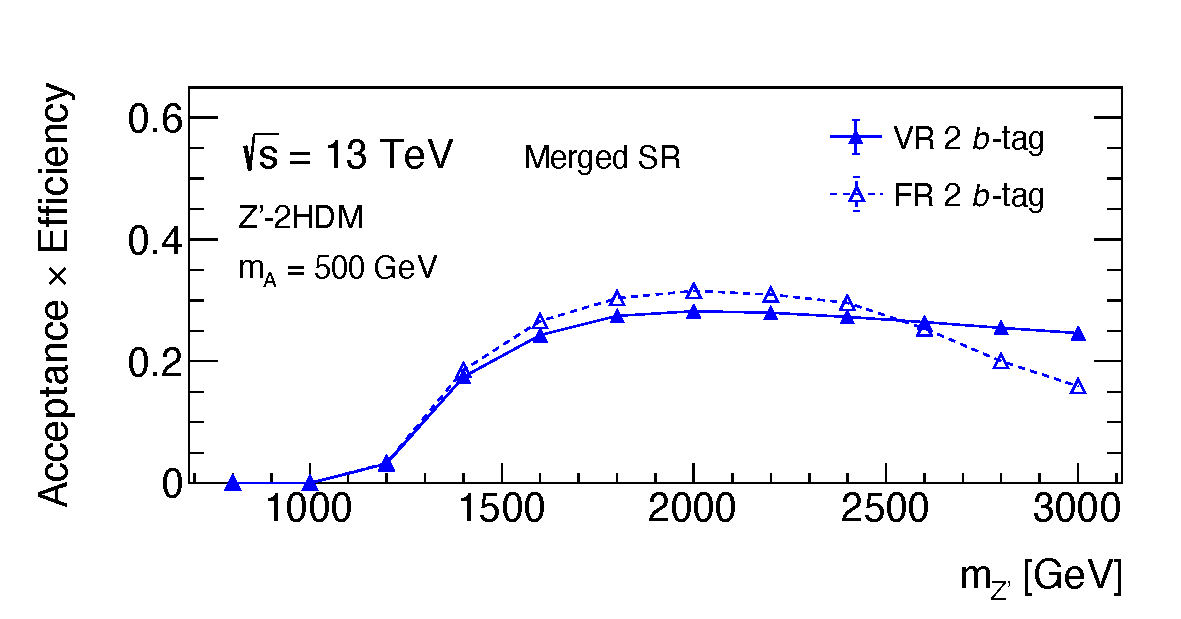
\includegraphics[width=0.95\textwidth]{figures/monoH/monoHaccXeffMerged.pdf}
  \caption{Product of detector acceptance \(\times\) selection efficiency in the signal region merged category shown in dependence of \mZp for a \zhdm signal sample with fixed \(\mA = \SI{500}{\giga\electronvolt}\). The performance for VR track jets (filled triangles, solid lines) is compared to that of FR track jets (open triangles, dashed lines).}
  \label{fig:monoH:selection:sr:accXeff-merged}
\end{figure}

No additional requirements to suppress the multijet background besides the baseline selection and \(\met > \SI{500}{\giga\electronvolt}\) are required for the merged category selection.

Similar as in the resolved category, the \ttbar background contribution is suppressed by dedicated requirements. Events containing \btagged VR track jets, which are not associated to the Higgs boson candidate, are rejected. Furthermore, events have to satisfy a requirement on the hadronic activity ratio \(H_{\text{T}}^{\text{merged}} < 0.57\). In the merged category, it is defined by the Higgs boson candidate \(\pt^{\text{J}}\) and the momenta of the central jets which do not overlap with the Higgs boson candidate \(\pt^{\text{j}_{i}}\) as
\begin{align}
H_{\text{T}}^{\text{merged}} = 1 - \frac{\text{Higgs candidate}}{\text{all jets}} = 1 - \frac{\pt^{\text{J}}}{\left(\sum_{i=1}^{N(\text{jets})}{\pt^{\text{j}_{i}}}+\pt^{\text{J}}\right)}.
\end{align}

Events with the Higgs boson candidate invariant mass in the range \(\SI{50}{\giga\electronvolt} < m_{J} < \SI{270}{\giga\electronvolt}\) are considered in the statistical analysis.

A summary of the SR selection requirements is presented in \Cref{tab:monoH:selection:sr:overview}.
\begin{table}[hbtp]
\caption{Signal region event selection requirements employed in the \(\met + \Hbb\) search.}
\label{tab:monoH:selection:sr:overview}
\centering
\begin{tabular}{ll}
\toprule
\multicolumn{2}{c}{\textbf{Common selection requirements}} \\
\midrule
\multicolumn{2}{c}{baseline selection requirements} \\
\multicolumn{2}{c}{multijet-suppression requirements} \\
\multicolumn{2}{c}{0 baseline \Pe and 0 baseline \Pgm} \\
\multicolumn{2}{c}{extended tau lepton veto} \\
\midrule
 \textbf{Resolved category} & \textbf{Merged category} \\
\midrule
\(\SI{150}{\giga\electronvolt} < \met < \SI{500}{\giga\electronvolt}\) & \(\met > \SI{500}{\giga\electronvolt}\) \\
\num{2} \btagged central jets & at least \num{1} large-radius jet \\
                        & associated with \num{2} \btagged VR track jets \\
\(\max\left\{\pt^{j1}, \pt^{j2}\right\} > \SI{45}{\giga\electronvolt}\) & no non-associated \btagged track jets \\
\( H_{\text{T}}^{\text{resolved}} < 0.37\) & \(H_{\text{T}}^{\text{merged}} < 0.57\) \\
\(\sum_{i}^{2(3)} \pt^{j_{i}} > \SI{120}{\giga\electronvolt} (\SI{150}{\giga\electronvolt})\) & \\
\(\mathcal{S} > 16\) &  \\
\(\Delta\varphi(\text{jet}_1,\text{jet}_2) < \SI{140}{\degree}\) &  \\
\(\Delta R(j_{1},j_{2}) < 1.8\) &  \\
\(\Delta\varphi(\met, \Ph) > \SI{120}{\degree}\) &  \\
\bottomrule
\end{tabular}
\end{table}

The complementarity of resolved and merged signal categories is demonstrated in \Cref{fig:accXeff-mergedresolved}.
The combined acceptance \(\times\) efficiency is shown by black filled points, and the acceptance \(\times\) efficiency of individual resolved and merged selections is indicated by open and filled blue triangles, respectively.
High signal efficiency is maintained over a broad range by employing both resolved and merged selection requirements.

\begin{figure}[hbt]
  \centering
  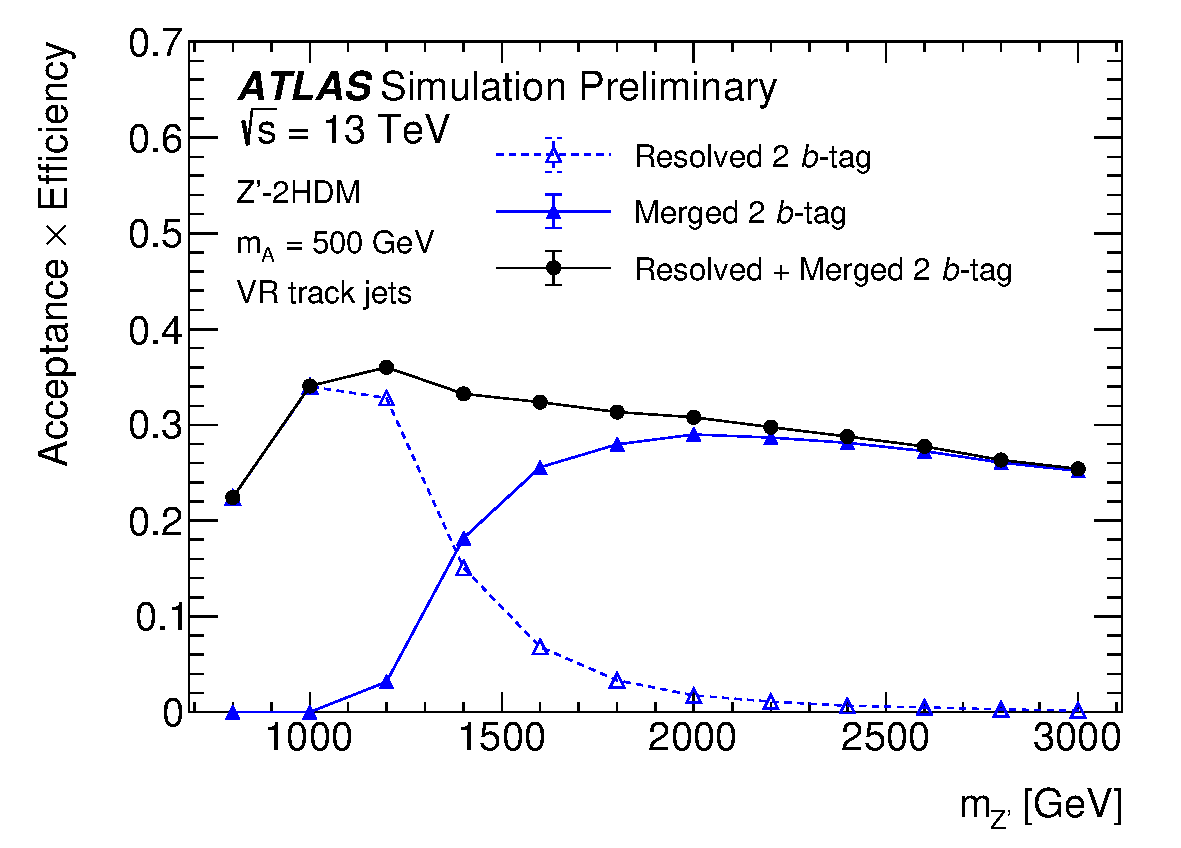
\includegraphics[width=.95\textwidth]{figures/monoH/results/fig_04.pdf}
  \caption{Product of detector acceptance \(\times\) selection efficiency for events with 2 \btagged jets as a function of \mZp for a \zhdm signal sample with fixed \(\mA = \SI{500}{\giga\electronvolt}\). The values obtained for the resolved category are shown in blue with open triangles and a dashed line, the ones for the merged category with filled triangles and a solid line. The combined selection efficiency is shown in black.}
  \label{fig:accXeff-mergedresolved}
\end{figure}


\section{Background estimation}
\label{sec:monoH:backgrounds}
The estimation of the dominant background processes in the \(\met + \Hbb\) search via MC simulation is improved by control region data. In contrast to the signal process, the dominant background processes have no characteristic peak in the Higgs candidate mass distributions. As the CRs have a high purity in the specific background processes, no additional \(m_{J}\) / \(m_{jj}\) information is used.

The normalisation parameters of the sub-dominant background processes are set to their predicted values based on theoretical predictions and can vary within the corresponding uncertainties.
The multijet background is found to be negligible based on a data-driven estimate, which is described in \Cref{sec:monoH:backgrounds:multijet}.

\subsection{1 muon control region}
\label{sec:monoH:backgrounds:cr1}
The 1 muon CR is defined to constrain \wjets and \ttbar processes. These background processes can contribute to the SR event selection by inefficiencies in the lepton reconstruction and muons outside of the detector acceptance. Consequently, the selected events contain exactly one tight signal muon, no additional baseline muons and no baseline electrons. The variable \metnomu is introduced, which is defined as the missing transverse momentum reconstructed by neglecting the muon in the event with the highest \pt. Events in the 1 muon CR are selected by \met triggers.

The other event selection requirements, such as the tau lepton veto, the requirements on the jet multiplicity and the event topology, are similar to the SR selection. In addition to the \metnomu information, the electrical charge of the muon is used in the statistical analysis to distinguish between \ttbar and \PW  + jets processes.
The fact that the LHC delivers proton-proton collisions results in a larger fraction of positively charged \PWp bosons produced in \wjets processes~\cite{Kom2010} because of the larger \Pqu parton luminosity with respect to the \Pqd parton luminosity (c.f. \Cref{fig:pp:pdfs:ct14}).
In contrast, the fractions of positively and negatively charged \PW bosons are equal in \ttbar processes.

The four \metnomu bins provide additional discrimination power, as the \ttbar background accumulates in the lower \metnomu bins, whereas the \wjets background accumulates in higher \metnomu bins.
A summary of the 1 muon CR selection requirements is presented in \Cref{tab:monoH:backgrounds:cr1:selections}.

\begin{table}[hbtp]
\caption{1 muon control region event selection requirements employed in the \(\met + \Hbb\) search.}
\label{tab:monoH:backgrounds:cr1:selections}
\centering
\begin{tabular}{ll}
\toprule
\multicolumn{2}{c}{\textbf{Common selection requirements}} \\
\midrule
\multicolumn{2}{c}{baseline selection requirements} \\
\multicolumn{2}{c}{multijet-suppression requirements} \\
\multicolumn{2}{c}{0 baseline \Pe, 1 tight signal \Pgm and no additional baseline \Pgm}\\
\multicolumn{2}{c}{extended tau lepton veto} \\
\midrule
\textbf{Resolved category} & \textbf{Merged category} \\
\midrule
\(\SI{150}{\giga\electronvolt} < \metnomu < \SI{500}{\giga\electronvolt}\) & \(\metnomu > \SI{500}{\giga\electronvolt}\) \\
\num{2} \btagged central jets & at least \num{1} large-radius jet \\
                        & associated with \num{2} \btagged VR track jets \\
\(\max\left\{\pt^{j1}, \pt^{j2}\right\} > \SI{45}{\giga\electronvolt}\) & no non-associated \btagged track jets \\
\( H_{\text{T}}^{\text{resolved}} < 0.37\) & \(H_{\text{T}}^{\text{merged}} < 0.57\) \\
\(\sum_{i}^{2(3)} \pt^{j_{i}} > \SI{120}{\giga\electronvolt} (\SI{150}{\giga\electronvolt})\) & \\
\(\mathcal{S}^{\text{no }\Pgm} > 16\) &  \\
\(\Delta\varphi(\text{jet}_1,\text{jet}_2) < \SI{140}{\degree}\) &  \\
\(\Delta R(j_{1},j_{2}) < 1.8\) &  \\
\(\Delta\varphi(\metnomu, \Ph) > \SI{120}{\degree}\) &  \\
\bottomrule
\end{tabular}
\end{table}

\subsection{2 lepton control region}
\label{sec:monoH:backgrounds:cr2}
The 2 lepton CR is designed to constrain the \zjets background using leptonically decaying \zjets events in the 2 lepton control region. The dilepton transverse momentum \ptll serves as a proxy of the missing transverse momentum.
The selected events contain either exactly two baseline electrons \HepProcess{\Pe \Pe} or exactly two baseline muons \HepProcess{\Pgm \Pgm}. At least one of the two electrons must satisfy the requirement \(\pt > \SI{27}{\giga\electronvolt}\). Similarly, at least one of the two muons must satisfy the requirements \(\pt > \SI{25}{\giga\electronvolt}\) and \(\abs{\eta} < 2.5\). Events containing two muons are only selected if these are of opposite charge. A similar requirement is not applied for events containing two electrons due to the higher rate of electron charge misidentification. Events in the 2 lepton CR are selected by single lepton triggers.

A requirement on the invariant mass of the dilepton system ensures high purity in \zjets processes by suppressing backgrounds with a non-resonantly produced lepton-pair. The requirement for events containing two muons is \(\SI{71}{\giga\electronvolt} < m_{\Pgm \Pgm} < \SI{106}{\giga\electronvolt}\), whereas for events containing two electrons the requirement is \(\SI{83}{\giga\electronvolt} < m_{\Pe\Pe} < \SI{99}{\giga\electronvolt}\), due to the better mass resolution of the EM calorimeter at high electron energies compared to the MS momentum resolution for high-\pt muons (c.f. \Cref{sec:experiment:ATLAS:calorimetry}).
No multijet-suppression requirements are part of the baseline selection for the 2 lepton CR, similarly the requirements on \(\Delta\varphi(j_{1},j_{2})\) and \(\Delta R(j_{1},j_{2})\) are not included in the 2 lepton CR selection.
Top quark background processes are suppressed by a requirement on the ratio of \met and the square root of the scalar sum of lepton and jet transverse momenta in the event, which is required to be \(\met / \sqrt{\sum (\pt^{\text{jets}} + \pt^{\text{leptons}})} < \SI{3.5}{\sqrt{\giga\electronvolt}}\).

Because of these selection requirements, the purity of the 2 lepton control region selection is sufficiently high to use the event yield in four \ptll bins directly as the observable in the statistical analysis.
A summary of the 2 lepton CR selection requirements is presented in \Cref{tab:monoH:backgrounds:cr2:selections}.

\begin{table}[hbtp]
\caption{2 lepton control region event selection requirements employed in the \(\met + \Hbb\) search.}
\label{tab:monoH:backgrounds:cr2:selections}
\centering
\begin{tabular}{ll}
\toprule
\multicolumn{2}{c}{\textbf{Common selection requirements}} \\
\midrule
\multicolumn{2}{c}{baseline selection requirements} \\
\multicolumn{2}{c}{exactly 2 baseline \Pe / \Pmu, among which 1 signal \Pe / \Pmu} \\
\multicolumn{2}{c}{extended tau lepton veto} \\
\multicolumn{2}{c}{\(\SI{71}{\giga\electronvolt} < m_{\Pgm \Pgm} < \SI{106}{\giga\electronvolt}\) or \(\SI{83}{\giga\electronvolt} < m_{\Pe\Pe} < \SI{99}{\giga\electronvolt}\)} \\
\multicolumn{2}{c}{\(\met / \sqrt{\sum (\pt^{\text{jets}} + \pt^{\text{leptons}})} < \SI{3.5}{\sqrt{\giga\electronvolt}}\)} \\
\midrule
\textbf{Resolved category} & \textbf{Merged category} \\
\midrule
\(\SI{150}{\giga\electronvolt} < \ptll < \SI{500}{\giga\electronvolt}\) & \(\ptll > \SI{500}{\giga\electronvolt}\) \\
\num{2} \btagged central jets & at least \num{1} large-radius jet \\
                        & associated with \num{2} \btagged VR track jets \\
\(\max\left\{\pt^{j1}, \pt^{j2}\right\} > \SI{45}{\giga\electronvolt}\) & no non-associated \btagged track jets \\
\( H_{\text{T}}^{\text{resolved}} < 0.37\) & \(H_{\text{T}}^{\text{merged}} < 0.57\) \\
\(\sum_{i}^{2(3)} \pt^{j_{i}} > \SI{120}{\giga\electronvolt} (\SI{150}{\giga\electronvolt})\) & \\
\(\Delta R(j_{1},j_{2}) < 1.8\) &  \\
\bottomrule
\end{tabular}
\end{table}


\subsection{Multijet background estimate}
\label{sec:monoH:backgrounds:multijet}
The multijet background is expected to be small in the SR resolved category due to the multijet-suppression requirements. It is expected to be negligible in the SR merged category as well as in the CRs due to the requirement of large \met and the additional lepton requirements, respectively.

The multijet background is estimated using a data-driven factorisation method, also referred to as ``ABCD'' method. The number of multijet events in the SR is determined by extrapolation from a multijet-enriched selection (region A), which is defined by the SR event selection with the two most powerful multijet-suppression requirements inverted, such that \(\min \Delta \varphi(\text{jets}_{1,2,3}, \met) < \SI{20}{\degree}\) and \(\mathcal{S} < 16\).

In this multijet-enriched selection, the number of multijet events is obtained from the difference between the data and the other simulated background processes. The corresponding distributions of the Higgs boson candidate mass \(m_{jj}\) are shown in \Cref{fig:monoH:backgrounds:multijet:templates}.

\begin{figure}[htbp]
  \centering
  \begin{subfigure}{0.45\textwidth}
    \centering
    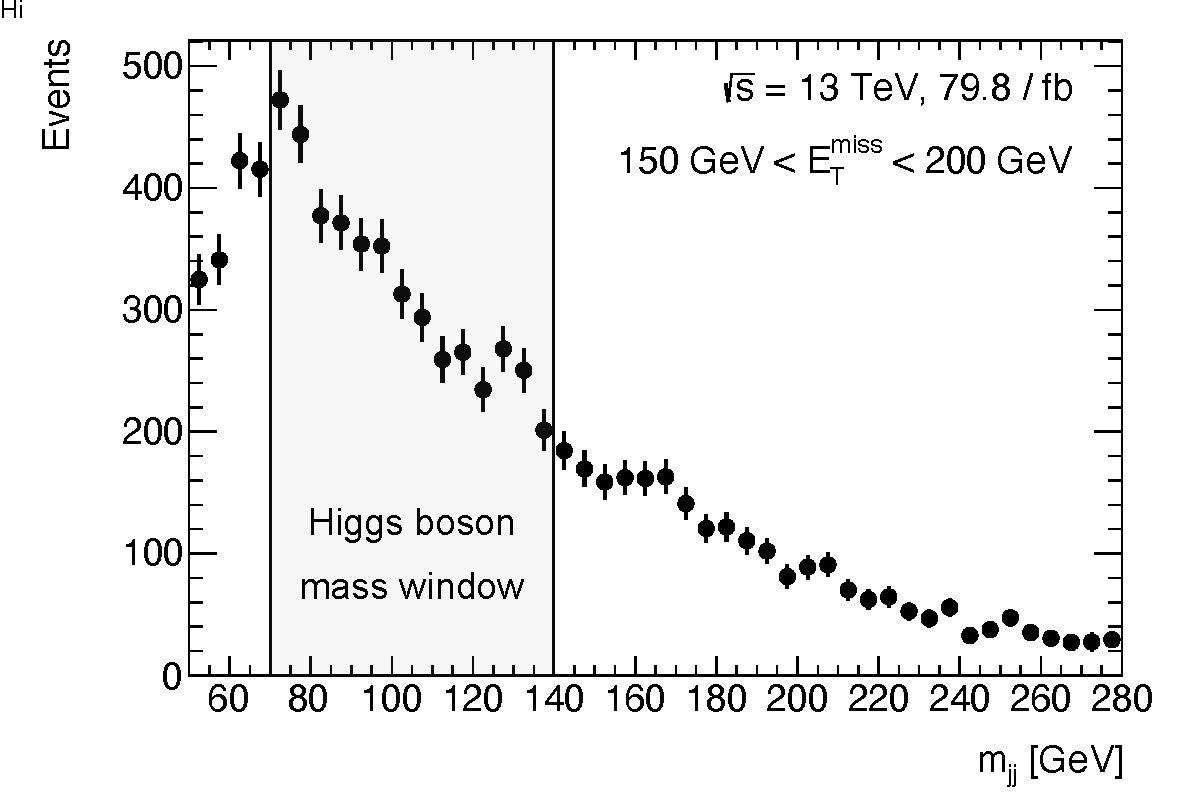
\includegraphics[width=0.95\textwidth]{figures/monoH/multijet/figures_multijetEstimate_template2b150200.pdf}
    \caption{\SI{150} < \met < \SI{200}{\giga\electronvolt}}
  \end{subfigure}%
  \begin{subfigure}{0.45\textwidth}
    \centering
    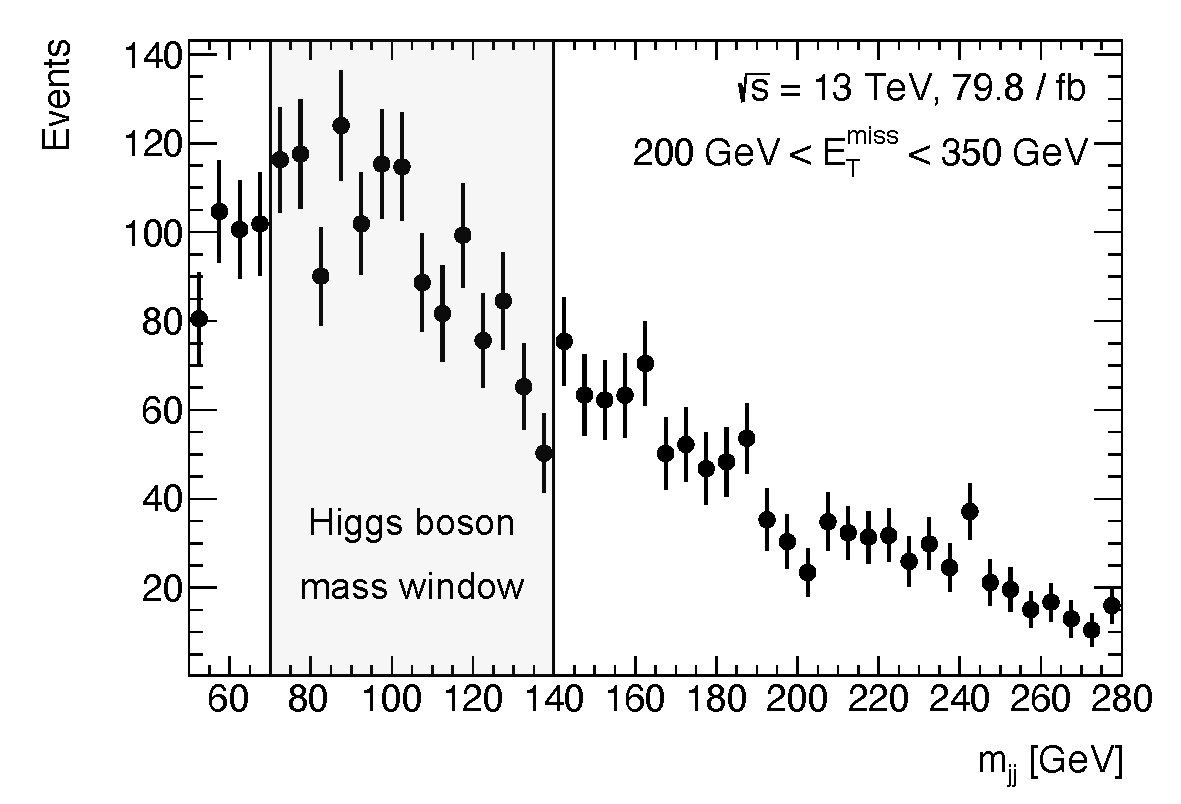
\includegraphics[width=0.95\textwidth]{figures/monoH/multijet/figures_multijetEstimate_template2b200350.pdf}
    \caption{\SI{200} < \met < \SI{350}{\giga\electronvolt}}
  \end{subfigure}
  \\
  \begin{subfigure}{0.45\textwidth}
    \centering
    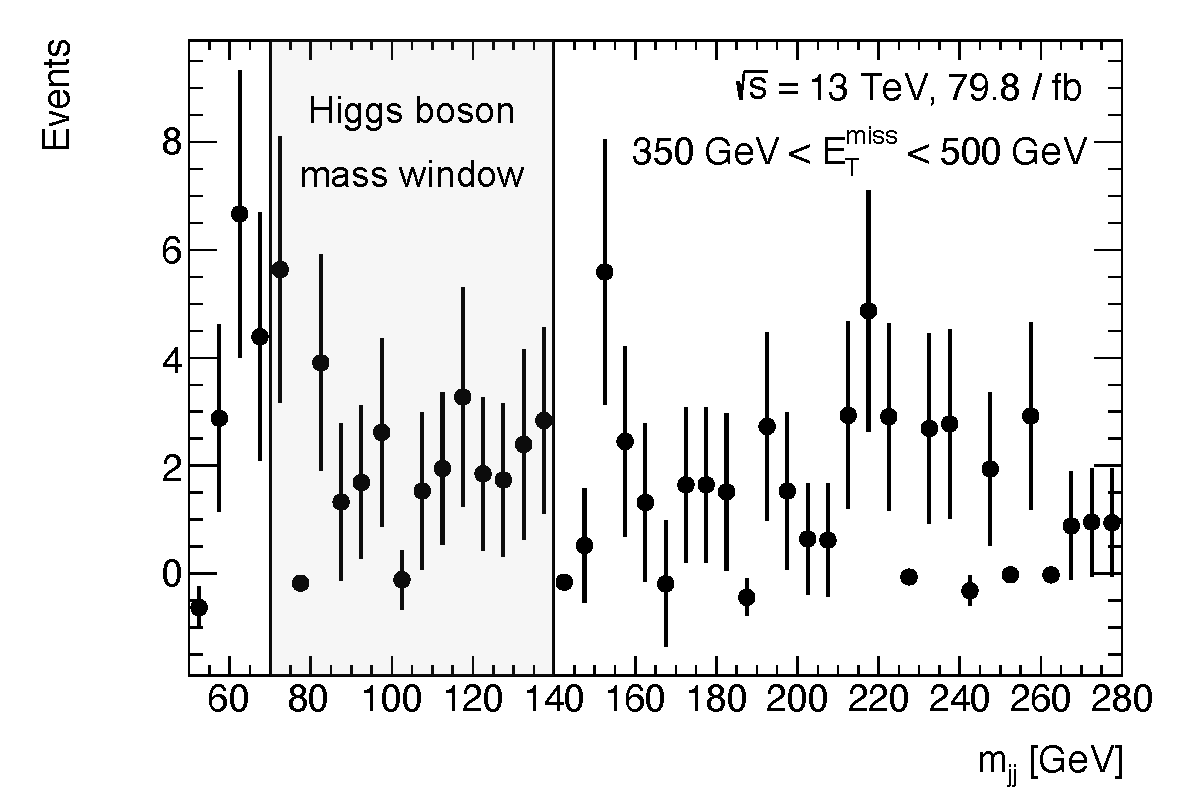
\includegraphics[width=0.95\textwidth]{figures/monoH/multijet/figures_multijetEstimate_template2b350500.pdf}
    \caption{\SI{350} < \met < \SI{500}{\giga\electronvolt}}
  \end{subfigure}
  \caption{Distributions of the Higgs boson candidate invariant mass \(m_{jj}\) for multijet background processes in the multijet-enriched region with 2 \btagged jets, obtained by subtracting all other simulated background processes from the data. The distributions are shown in the bins \(\SI{150}{\giga\electronvolt} < \met < \SI{200}{\giga\electronvolt}\) (left), \(\SI{150}{\giga\electronvolt} < \met < \SI{200}{\giga\electronvolt}\) (right), \(\SI{150}{\giga\electronvolt} < \met < \SI{200}{\giga\electronvolt}\) (bottom). The error bars represent the statistical uncertainty only.}
  \label{fig:monoH:backgrounds:multijet:templates}
\end{figure}

The multijet event yield in the SR (D) can be estimated by correcting for the efficiency of the \(\min \Delta \varphi(\text{jets}_{1,2,3}, \met)\) and \(\mathcal{S}\) selection requirements.
To this end, two additional selections --- region B and region C --- are defined, in which only one of the two selection requirements is inverted.
Together with the multijet-enriched selection and the SR, four regions are defined in total, which is illustrated in \Cref{fig:monoH:backgrounds:multijet:procedure}.

\begin{figure}[htbp]
  \centering
  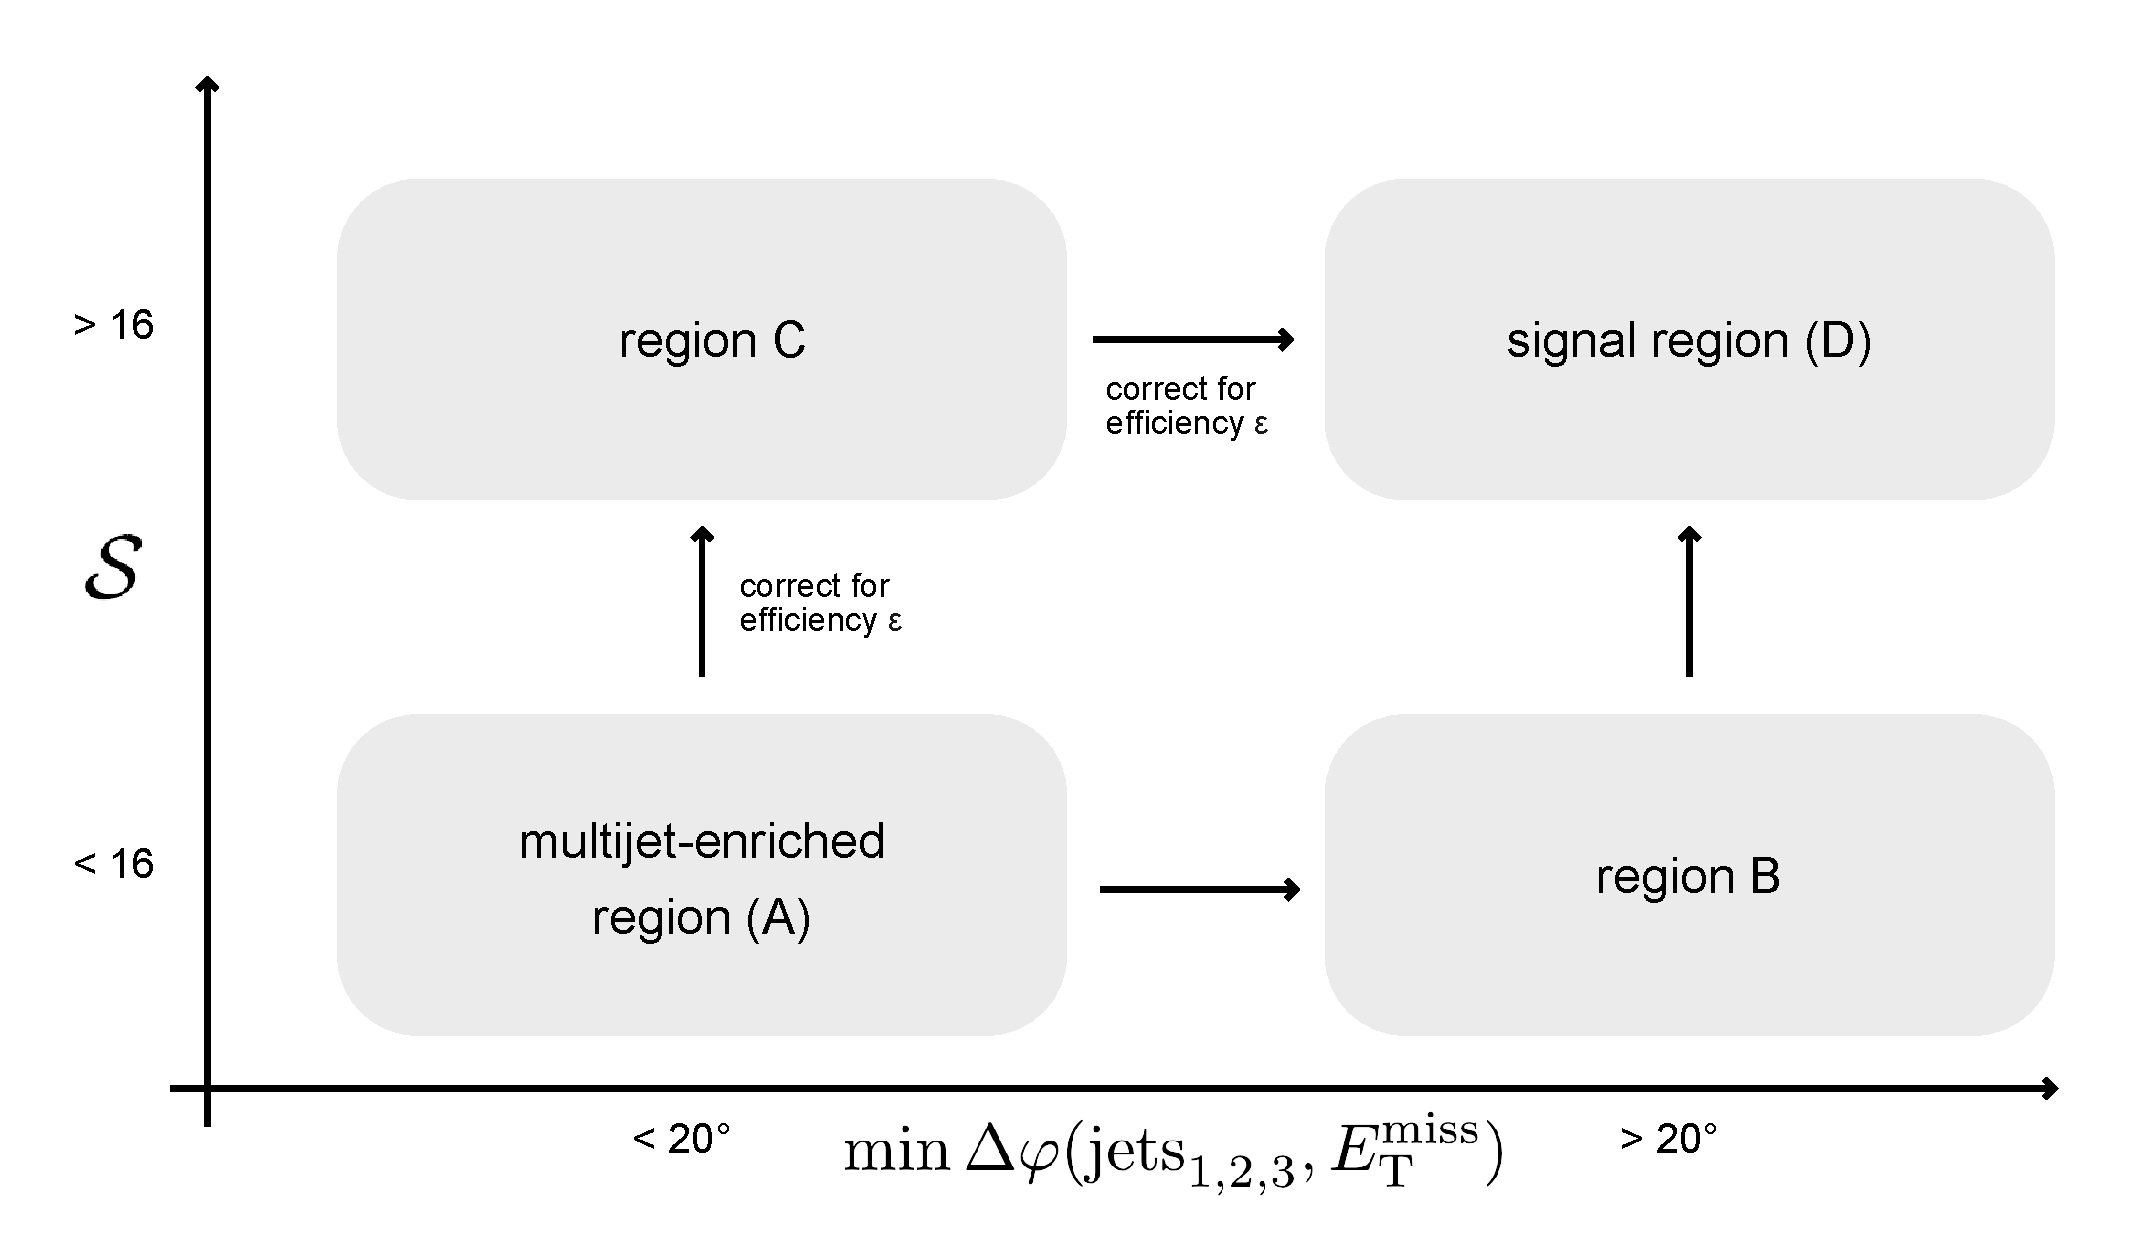
\includegraphics[width=0.95\textwidth]{figures/monoH/monoHmultijetprocedure.pdf}
  \caption{Sketch of the regions used in the multijet background estimate based on a factorisation method. The multijet-enriched region A is defined by inverting both the \(\min \Delta \varphi(\text{jets}_{1,2,3}, \met)\) and \(\mathcal{S}\) requirements. The regions B and C are defined by inverting only one of those requirements, whereas both requirements are applied in the signal region D.}
  \label{fig:monoH:backgrounds:multijet:procedure}
\end{figure}

If \(\min \Delta \varphi(\text{jets}_{1,2,3}, \met)\) and \(\mathcal{S}\) are not strongly correlated, the amount of multijet events in the signal region can be estimated as
\begin{align}
\hat{N}_{\text{D} (\mathcal{S} > 16, \min \Delta \varphi > \SI{20}{\degree})} = \frac{N_{\text{B} (\mathcal{S} < 16, \min \Delta \varphi > \SI{20}{\degree})}}{N_{\text{A} (\mathcal{S} < 16, \min \Delta \varphi < \SI{20}{\degree})}} \times N_{\text{C} (\mathcal{S} > 16, \min \Delta \varphi < \SI{20}{\degree})},
\end{align}
where \(N_{R (\mathcal{S}, \min \Delta \varphi})\) denotes the number of multijet events in the respective region \(R\), which is obtained as the difference between the data and the other simulated background processes.

\Cref{fig:monoH:backgrounds:multijet:correlation-metsig} compares the shape of \(\mathcal{S}\) for different selections in \(\min \Delta \varphi(\text{jets}_{1,2,3}, \met)\). As the \(\mathcal{S}\) shape is independent of \(\min \Delta \varphi(\text{jets}_{1,2,3}, \met)\), the assumption of the two variables being uncorrelated is justified.
The corresponding two-dimensional distributions of \(\mathcal{S}\) and \(\min \Delta \varphi(\text{jets}_{1,2,3}, \met)\) are shown in \Cref{fig:monoH:backgrounds:multijet:correlation}.

\begin{figure}[htbp]
  \centering
  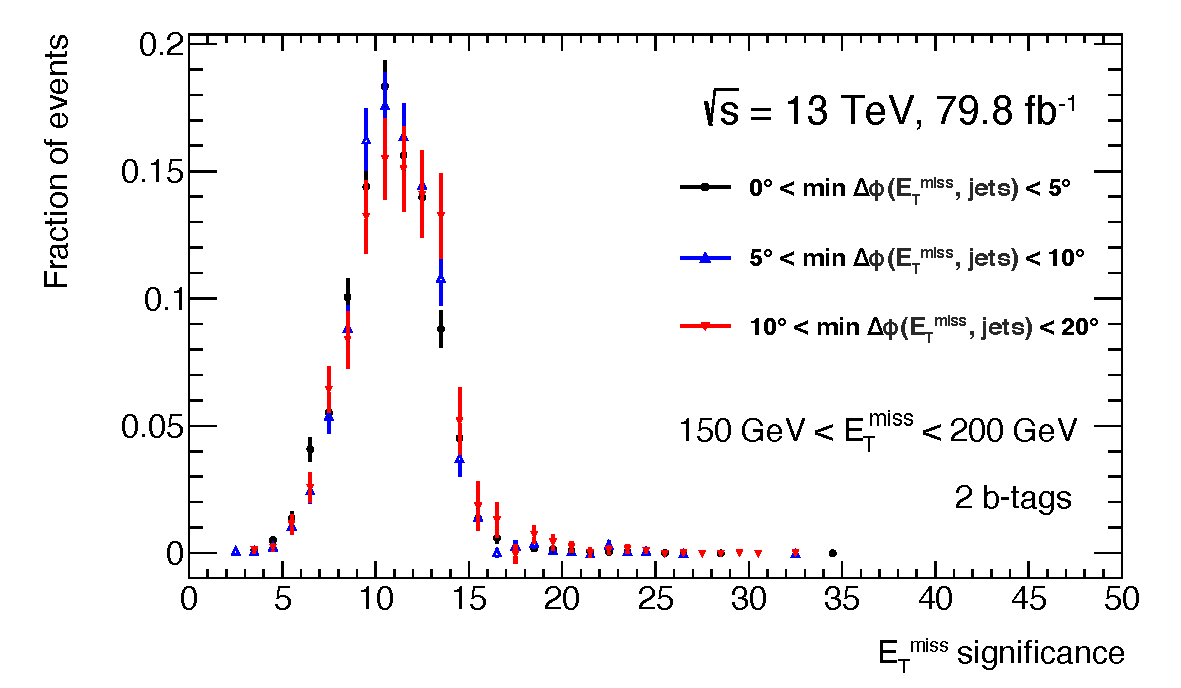
\includegraphics[width=0.75\textwidth]{figures/monoH/multijet/monoHmultijet_correlation_metsig.pdf}
  \caption{Shape of the object-based \met significance \(\mathcal{S}\) shown for the difference between the data and the other simulated background processes in different selections of \(\min \Delta \varphi(\text{jets}_{1,2,3}, \met)\). The selected events have two \btagged jets and satisfy \(\SI{150}{\giga\electronvolt} < \met < \SI{200}{\giga\electronvolt}\).}
  \label{fig:monoH:backgrounds:multijet:correlation-metsig}
\end{figure}

\begin{figure}[htbp]
  \centering
  \begin{subfigure}{1.\textwidth}
    \centering
    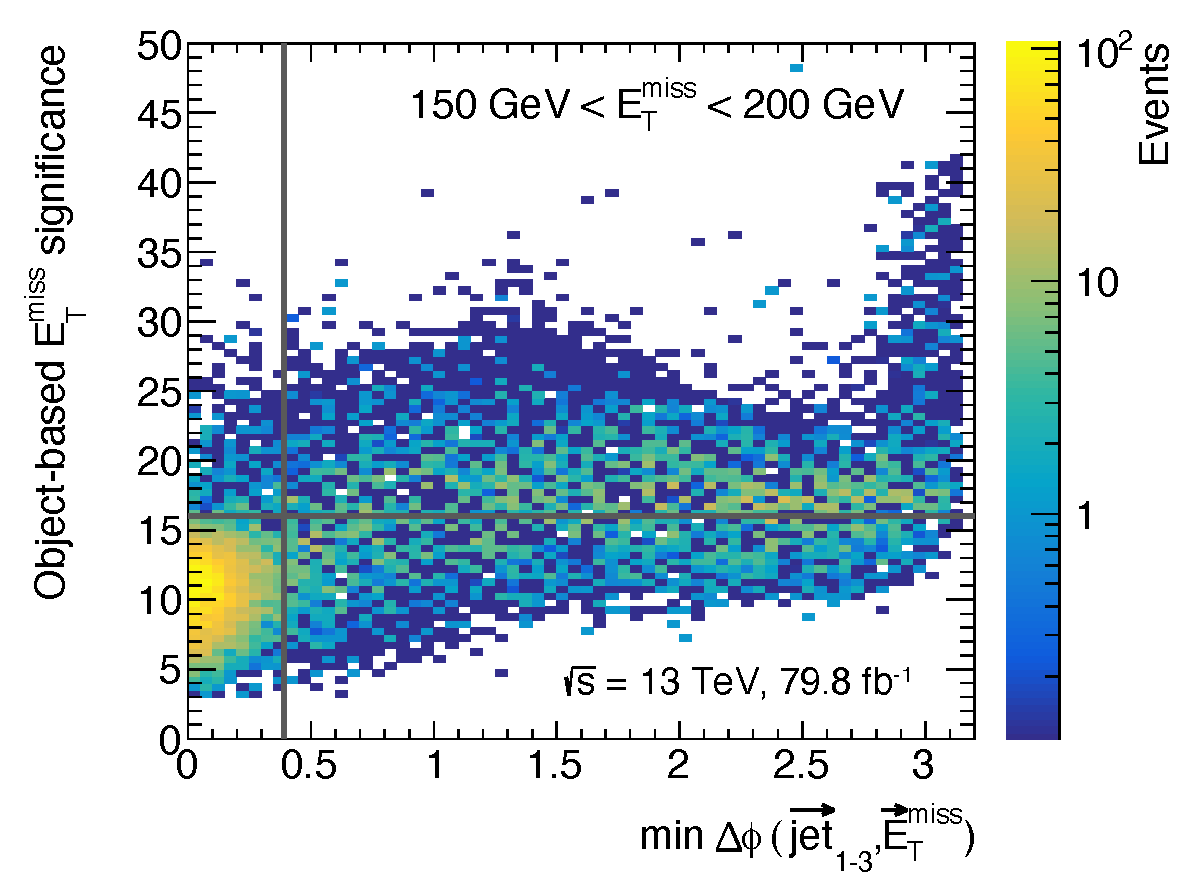
\includegraphics[width=0.6\textwidth]{figures/monoH/multijet/monoHmultijet_correlation150200.pdf}
    \caption{\SI{150} < \met < \SI{200}{\giga\electronvolt}}
  \end{subfigure}
  \\
  \begin{subfigure}{1.\textwidth}
    \centering
    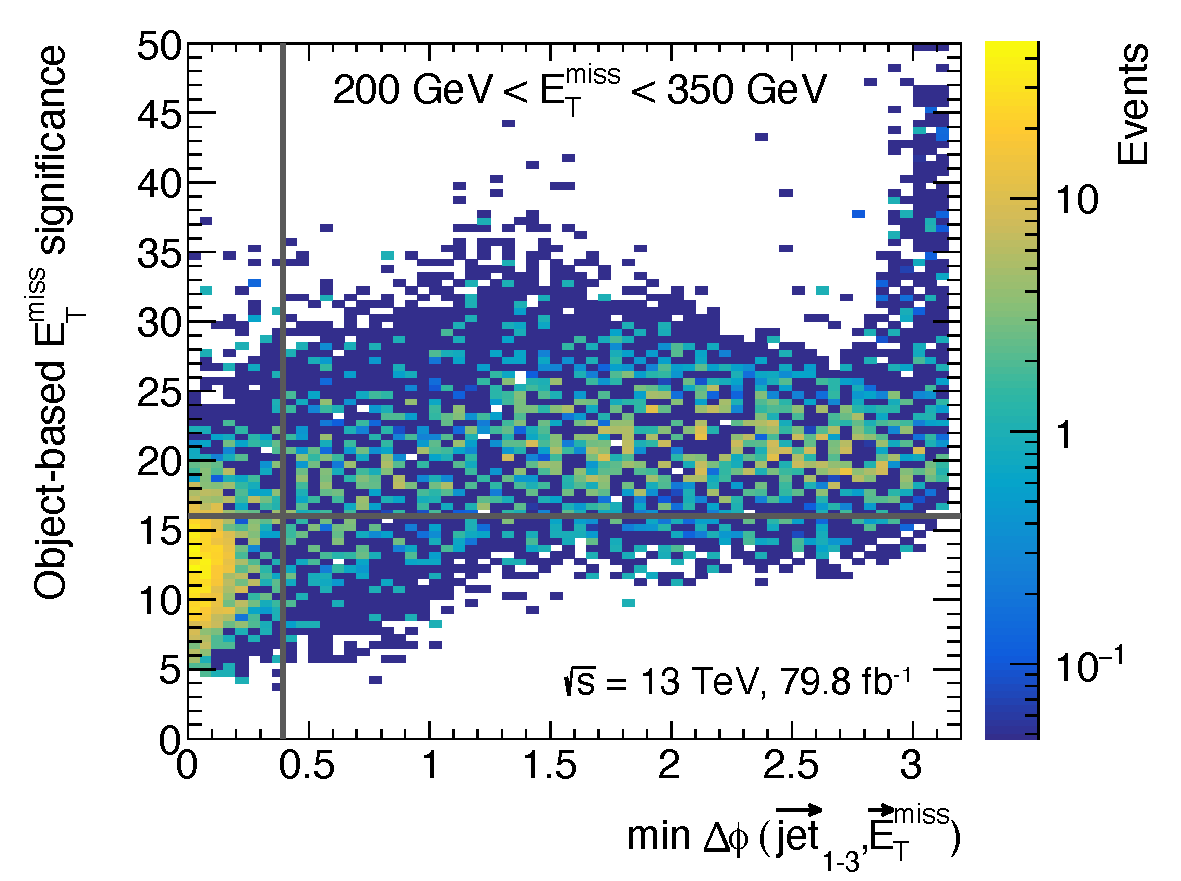
\includegraphics[width=0.6\textwidth]{figures/monoH/multijet/monoHmultijet_correlation200350.pdf}
    \caption{\SI{200} < \met < \SI{350}{\giga\electronvolt}}
  \end{subfigure}
  \\
  \begin{subfigure}{1.\textwidth}
    \centering
    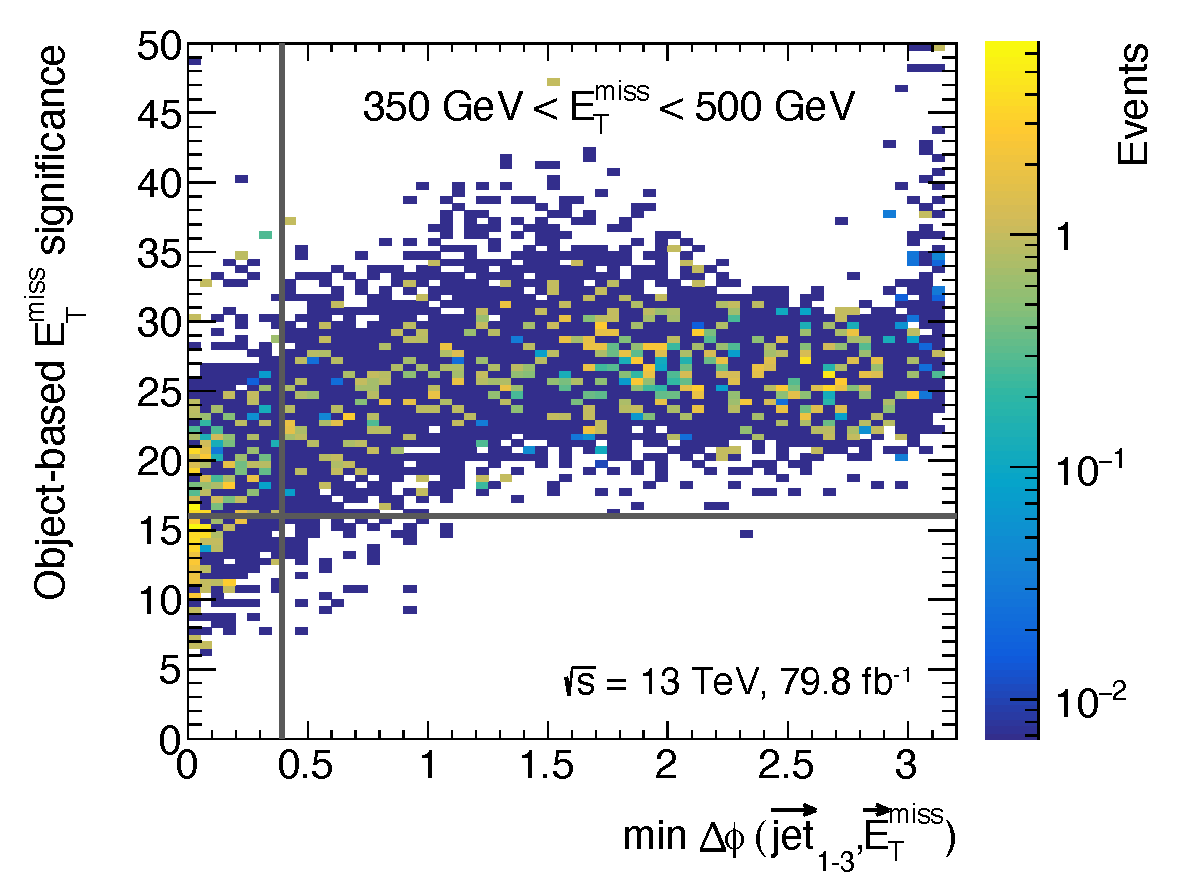
\includegraphics[width=0.6\textwidth]{figures/monoH/multijet/monoHmultijet_correlation350500.pdf}
    \caption{\SI{350} < \met < \SI{500}{\giga\electronvolt}}
  \end{subfigure}
  \caption{Two-dimensional distributions of \(\mathcal{S}\) and \(\min \Delta \varphi(\text{jets}_{1,2,3}, \met)\) for multijet background processes, obtained by subtracting all other simulated background processes from the data. The grey lines indicate the regions used in the multijet estimate. The distributions are shown in the bins \(\SI{150}{\giga\electronvolt} < \met < \SI{200}{\giga\electronvolt}\) (left), \(\SI{150}{\giga\electronvolt} < \met < \SI{200}{\giga\electronvolt}\) (right), \(\SI{150}{\giga\electronvolt} < \met < \SI{200}{\giga\electronvolt}\) (bottom).}
  \label{fig:monoH:backgrounds:multijet:correlation}
\end{figure}

The estimate is performed by excluding events in the Higgs boson mass window \(\SI{70}{\giga\electronvolt} < m_{jj} < \SI{140}{\giga\electronvolt}\) to avoid the contamination by potential signals.
The corresponding event yields for the observed data and the total simulated background processes (excluding the multijet background) are shown in \Cref{tab:monoH:backgrounds:multijet:results}. The multijet background reported in the regions A, B, and C is the difference between the data and the simulated background processes.
The corresponding errors account only for the statistical uncertainty.


\begin{table}[hbtp]
\caption{Event yields of the observed data, the simulated background processes, and their difference in the regions A, B, C, and D.}
\label{tab:monoH:backgrounds:multijet:results}
\centering
\resizebox{\textwidth}{!}{%
\sisetup{round-mode=figures, round-precision=2,
         retain-explicit-plus=true, group-digits=integer, group-minimum-digits=4}%
\begin{tabular}{ll %
S[table-format=4.1, table-number-alignment=right, round-mode=figures, round-precision=3]@{$\,\pm\,$}%
S[table-format=2.1, table-number-alignment=right, round-mode=figures, round-precision=2]@{\quad}%
S[table-format=4.1, table-number-alignment=right, round-mode=figures, round-precision=3]@{$\,\pm\,$}%
S[table-format=2.1, table-number-alignment=right, round-mode=figures, round-precision=2]@{\quad}%
S[table-format=3.1, table-number-alignment=right, round-mode=figures, round-precision=3]@{$\,\pm\,$}%
S[table-format=2.1, table-number-alignment=right, round-mode=figures, round-precision=2]@{\quad}%
S[table-format=4.1, table-number-alignment=right, round-mode=figures, round-precision=3]@{$\,\pm\,$}%
S[table-format=2.1, table-number-alignment=right, round-mode=figures, round-precision=2]@{\quad}}
\toprule %
Sample & \met range & \multicolumn{2}{c}{\(N_{\text{A}}\)} & \multicolumn{2}{c}{\(N_{\text{B}}\)} & \multicolumn{2}{c}{\(N_{\text{C}}\)} & \multicolumn{2}{c}{\(N_{\text{D}}\)} \\
\midrule
Data & \SIrange{150}{200}{\giga\electronvolt}       & 4573 & 68 & 3452 &  59 & 129 & 11 & 7698 & 88   \\
Other bkg. & \SIrange{150}{200}{\giga\electronvolt} &  595 & 13 & 2435 &  28 &  50 &  3 & 6397 & 45   \\
Multijet & \SIrange{150}{200}{\giga\electronvolt}   & 3978 & 69 & 1017 &  65 &  79 & 12 & \multicolumn{2}{c}{\text{n.a.}} \\
\\
Data & \SIrange{200}{350}{\giga\electronvolt}       & 1705 & 41 &  381 &  20 & 355 & 19 & 5429 & 74   \\
Other bkg. & \SIrange{200}{350}{\giga\electronvolt} &  282 &  9 &  317 &  10 & 174 &  7 & 4731 & 36   \\
Multijet & \SIrange{200}{350}{\giga\electronvolt}   & 1423 & 42 &   64 &  22 & 181 & 20 & \text{n.a.} \\
\\
Data & \SIrange{350}{500}{\giga\electronvolt}       &   66 &  8 &  1   & 1   &  94 & 10 &  484 & 22   \\
Other bkg. & \SIrange{350}{500}{\giga\electronvolt} &    9 &  1 &  0.9 & 0.2 &  52 &  4 &  434 &  9   \\
Multijet & \SIrange{350}{500}{\giga\electronvolt}   &   57 &  8 &  0.1 & 1   &  42 & 11 & \text{n.a.} \\
\bottomrule %
\end{tabular}}
\end{table}

The estimated multijet event yield in the SR Higgs boson mass side-band is
\begin{itemize}
  \item \num{20 \pm 3.3} events for \(\SI{150}{\giga\electronvolt} < \met < \SI{200}{\giga\electronvolt}\),
  \item \num{8 \pm 2.9} events for \(\SI{200}{\giga\electronvolt} < \met < \SI{350}{\giga\electronvolt}\), and
  \item \num{0 \pm 0.8} events for \(\SI{350}{\giga\electronvolt} < \met < \SI{500}{\giga\electronvolt}\).
\end{itemize}
It is substantially smaller than the statistical uncertainty of the observed data and thus can be safely neglected.

In order to draw a similar conclusion for the full \(m_{jj}\) range in the SR, the predicted multijet event yield in the SR Higgs boson mass side-bands needs to be corrected for the events in the Higgs boson mass window.
A rough estimate for this correction factor is obtained from the multijet \(m_{jj}\) distributions in the multijet-enriched region D, which are shown in \Cref{fig:monoH:backgrounds:multijet:templates}. Their shape corresponds to that of the multijet background in the SR, although the latter is afflicted with sizeable statistical uncertainty, as shown in \Cref{fig:monoH:backgrounds:multijet:mass-shape}.

\begin{figure}[htbp]
  \centering
  \begin{subfigure}{0.45\textwidth}
    \centering
    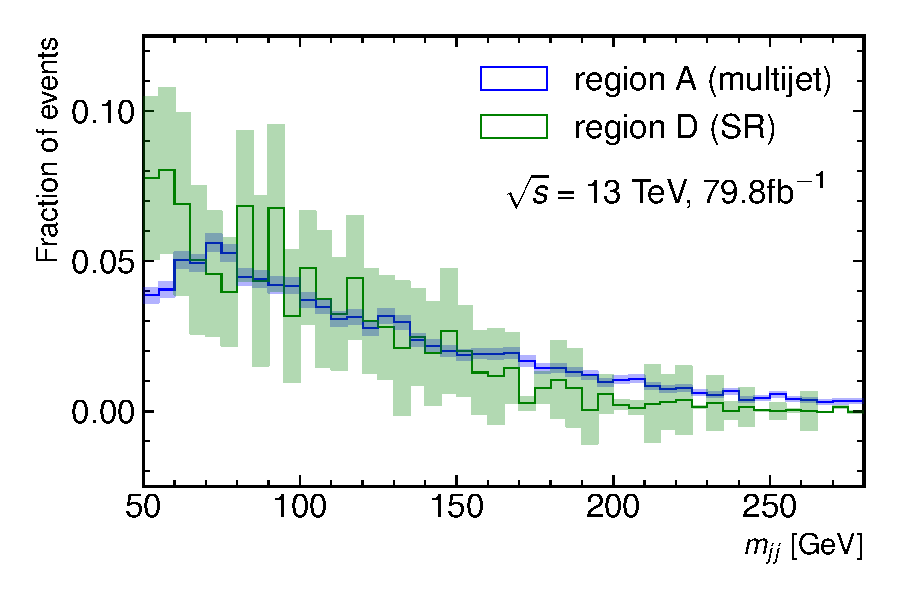
\includegraphics[width=0.95\textwidth]{figures/monoH/multijet/monoHmultijet_correlation-mass_SR_Resolved_150_200_2b.pdf}
    \caption{\SI{150} < \met < \SI{200}{\giga\electronvolt}}
  \end{subfigure}%
  \begin{subfigure}{0.45\textwidth}
    \centering
    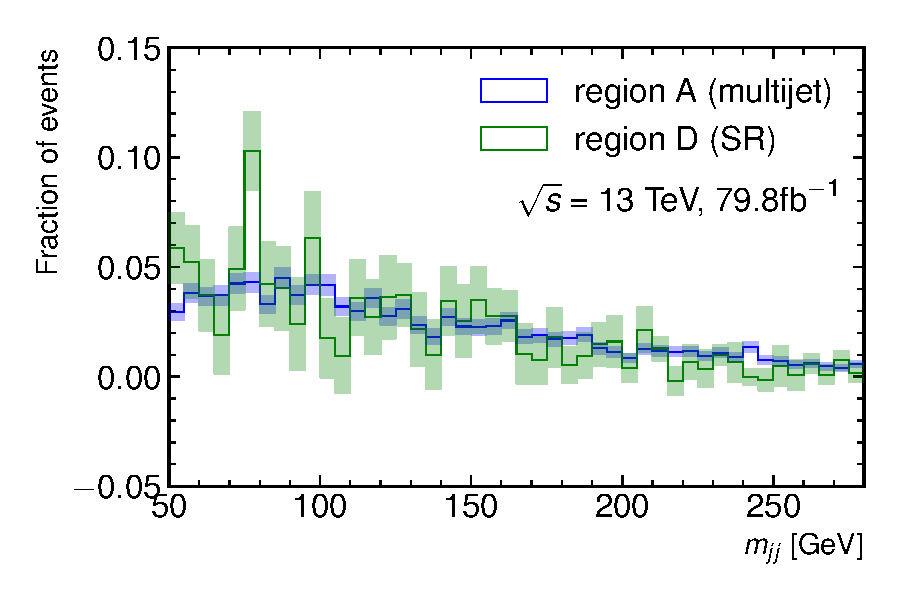
\includegraphics[width=0.95\textwidth]{figures/monoH/multijet/monoHmultijet_correlation-mass_SR_Resolved_200_350_2b.pdf}
    \caption{\SI{200} < \met < \SI{350}{\giga\electronvolt}}
  \end{subfigure}
  \\
  \begin{subfigure}{0.45\textwidth}
    \centering
    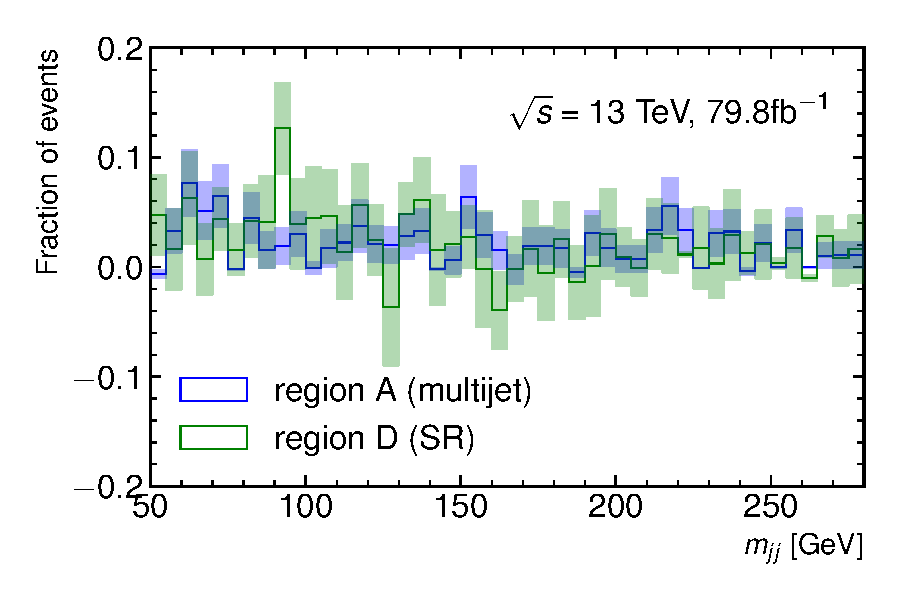
\includegraphics[width=0.95\textwidth]{figures/monoH/multijet/monoHmultijet_correlation-mass_SR_Resolved_350_500_2b.pdf}
    \caption{\SI{350} < \met < \SI{500}{\giga\electronvolt}}
  \end{subfigure}
  \caption{Comparison of the shapes of the Higgs boson candidate invariant mass \(m_{jj}\) for the multijet background in the multijet-enriched region and the signal region. The shapes are obtained by subtracting all other simulated background processes from the data. The distributions are shown in the bins \(\SI{150}{\giga\electronvolt} < \met < \SI{200}{\giga\electronvolt}\) (left), \(\SI{150}{\giga\electronvolt} < \met < \SI{200}{\giga\electronvolt}\) (right), \(\SI{150}{\giga\electronvolt} < \met < \SI{200}{\giga\electronvolt}\) (bottom). The error bands represent the statistical uncertainty only.}
  \label{fig:monoH:backgrounds:multijet:mass-shape}
\end{figure}

Therefore, the correction factor is obtained in the multijet-enriched region D as the ratio of the multijet events in the full mass range and the multijet events outside of the Higgs boson mass window.
Thus, the total predicted multijet yield is smaller than
\begin{itemize}
	\item \num{38 \pm 17} events for \(\SI{150}{\giga\electronvolt} < \met < \SI{200}{\giga\electronvolt}\),
	\item \num{14 \pm 22} events for \(\SI{200}{\giga\electronvolt} < \met < \SI{350}{\giga\electronvolt}\), and
	\item \num{0 \pm 80} events for \(\SI{350}{\giga\electronvolt} < \met < \SI{500}{\giga\electronvolt}\).
\end{itemize}

Although the prediction in the highest \met bin is afflicted with large statistical uncertainty, an extrapolation from the two lower \met bins shows that it is negligible.
Multijet processes typically decrease exponentially in \met. Therefore, comparing the event yields between bins shows that multijet background falls off much steeper than the observed data outside the Higgs peak.

The estimated total multijet background event yield in the SR is substantially smaller than the statistical uncertainty on the total data. Therefore, it is neglected in the background model.


\section{Systematic uncertainties}
\label{sec:monoH:systematics}
Systematic uncertainties arise from the biases in the reconstruction of physics objects and the description of the signal and background processes using MC simulation. The experimental systematic uncertainties are described in \Cref{sec:monoH:systematics:experimental}, while the theoretical systematic uncertainties are described in \Cref{sec:monoH:systematics:theoretical}.

\subsection{Experimental systematic uncertainties}
\label{sec:monoH:systematics:experimental}
The experimental systematic uncertainties in the \(\met + \Hbb\) search, which arise from biases in the reconstruction of physics objects, resemble those of the \(\met + \Vqq\) search. The shared uncertainties include the trigger uncertainties, the uncertainties related to the pile-up modelling, the uncertainties on the reconstruction and calibration of electrons, muons, small-radius jets, \btagging uncertainties, and the \met soft term uncertainties. The differences in the experimental uncertainties are listed below.

\begin{itemize}
  \item \textbf{Luminosity.} The uncertainty on the measurement of the integrated luminosity is \SI{2.0}{\percent}~\cite{ATLAS-CONF-2019-021}.
  \item \textbf{Large-radius jets.} The large-radius jet uncertainties are defined for their energy and mass resolution, and their mass and \pt scale. The latter uncertainties are described by four components, which account for the residual difference between data and MC simulation, the fragmentation modelling, uncertainties related to the use of tracking information, and the total statistical uncertainty in the calibration. The uncertainties on the resolution are described by one component for the jet energy and mass, each.
\end{itemize}


\subsection{Theoretical systematic uncertainties}
\label{sec:monoH:systematics:theoretical}
The theoretical systematic uncertainties arise from specific choices of event generators, PDF sets, parton shower modelling, and values of the renormalisation and factorisation scales in the modelling of signal and background processes. The evaluation of the theoretical systematic uncertainties follows the same strategy as described in Ref.~\cite{HIGG-2018-04}.

In the description of the \vjets background processes, the contributions of different jet flavour are accounted for individually. The simulated \vjets background events are categorised as \HepProcess{V + \Pqb \Pqb}, \HepProcess{V + \Pqb \Pqc}, \HepProcess{V + \Pqb l}, \HepProcess{V + \Pqc\Pqc}, \HepProcess{V + \Pqc l}, and \HepProcess{V + ll}, where \(l \in \{\Pqu, \Pqd, \Pqs, \Pg\}\) denotes light flavour jets. The heavy-flavour processes \HepProcess{V + \Pqb \Pqb}, \HepProcess{V + \Pqb \Pqc}, and \HepProcess{V + \Pqb l}, \HepProcess{V + \Pqc\Pqc} are grouped and referred to as \HepProcess{V + \text{hf}}.

The total normalisations of the dominant background processes --- \ttbar, \HepProcess{\PZ + \text{hf}}, and \HepProcess{\PW + \text{hf}} --- are determined by the control region data.
The relative contributions of the individual heavy-flavour processes are allowed to change within their theoretical uncertainties. These uncertainties are determined by comparing the nominal \SHERPA MC samples to alternative samples generated with \MADGRAPHV{5} (c.f. \Cref{sec:monoV:systematics:theoretical}) and taking the largest difference as the uncertainty.
The normalisation of the \zjets and \wjets background processes is decorrelated by \SI{20}{\percent} among SR and CRs, as the varied kinematic distributions of leptons due to scale and PDF uncertainties introduce selection efficiency biases due to the limited detector acceptance for leptons. These uncertainties have been studied in Ref.~\cite{HIGG-2018-04} and have been adopted here.

The normalisations of the sub-dominant background processes --- \HepProcess{V + \Pqc l}, \HepProcess{V + ll}, single top quark production, \VHbb production, and diboson processes ---are constrained by the normalisation uncertainties, which are estimated from theoretical expectations. The normalisation uncertainties of single top-quark production include scale variations and PDF uncertainties, whereas the diboson uncertainties include scale variations as well as parton shower uncertainties. The \VHbb uncertainty is taken from the ATLAS measurement presented in Ref.~\cite{HIGG-2016-29}. The normalisation uncertainties are listed in \Cref{tab:monoH:systematics:theoretical:norm}.

\begin{table}[hbtp]
\caption{Theoretical systematic uncertainties on the normalisation of background processes in the \(\met + \Hbb\) search.}
\label{tab:monoH:systematics:theoretical:norm}
\centering
\begin{tabular}{l r}
\toprule
Process & Uncertainty \\
\midrule
Ratio of \HepProcess{V + \Pqb\Pqc} / \HepProcess{V + \text{heavy flavour}} & \SI{20}{\percent}\\
Ratio of \HepProcess{V + \Pqb l} / \HepProcess{V + \text{heavy flavour}} & \SI{20}{\percent}\\
Ratio of \HepProcess{V + \Pqc\Pqc} / \HepProcess{V + \text{heavy flavour}} & \SI{20}{\percent}\\
\midrule
Ratio of \HepProcess{\PW + \text{hf}} in SR and 1 muon CR & \SI{20}{\percent}\\
Ratio of \HepProcess{\PZ + \text{hf}} in SR and 2 lepton CR & \SI{20}{\percent}\\
\midrule
\HepProcess{V + \Pqc l} & \SI{30}{\percent} \\
\HepProcess{V + l} & \SI{10}{\percent} \\
\midrule
Single top quark (\(s\)-channel) & \SI{4.6}{\percent} \\
Single top quark (\(t\)-channel) & \SI{4.4}{\percent} \\
Single top quark (\(\PW t\)-process) & \SI{6.2}{\percent} \\
\midrule
\HepProcess{\PW \PW} & \SI{25}{\percent} \\
\HepProcess{\PW \PZ} & \SI{26}{\percent} \\
\HepProcess{\PZ \PZ} & \SI{20}{\percent} \\
\VHbb & \SI{30}{\percent} \\
\bottomrule
\end{tabular}
\end{table}

In addition, shape uncertainties on both the \met (or \metnomu / \ptll) and Higgs boson candidate invariant mass distributions are considered, which are obtained by comparing samples generated with different event generator settings, as well as comparisons to events in data in a selection enriched in \zjets events.
Their estimation follows the procedure described in \Cref{sec:monoV:systematics:theoretical}.

The theoretical uncertainties for the dark matter signals in the \zhdm model are estimated by variations in the event generation and comparing the event yields at particle level neglecting detector effects. The uncertainties are defined in three components.
\begin{itemize}
  \item The \textbf{scale} uncertainties are estimated by varying the renormalisation scale \muR and factorisation scale \muF coherently by factors of \num{0.5} and \num{2} on an event-by-event basis. The largest variation with respect to the nominal value is taken as the scale uncertainty.
  \item The \textbf{PDF} uncertainty is estimated by replacing the nominal \textsc{NNPDF30LO} PDF set with the alternative \textsc{MSTW2008LO}~\cite{Martin2009} and \textsc{CTEQ6L1}~\cite{Pumplin:2002vw} PDF sets. The largest deviation between the nominal and alternative PDF sets is taken as the signal PDF uncertainty.
  \item The \textbf{tune} uncertainty is estimated by varying the amounts of initial state radiation, final state radiation, and multi-parton interactions.
\end{itemize}
The average size of the signal acceptance uncertainties is below \SI{1}{\percent}, except for a few signal mass points with lower acceptance.
The signal acceptance uncertainties are correlated over the \met bins by considering a single nuisance parameter for each type of systematic uncertainty.


\section{Statistical model}
\label{sec:monoH:model}
The statistical model is based on the likelihood function \Cref{eq:methods:statistics:likelihood}. The profile likelihood fit is based on the \met bins and the invariant mass of the Higgs boson candidate in the SR, the muon charge and the \metnomu bins in the 1 muon CR, and the \ptll bins in the  2 lepton CR.
While the Higgs boson candidate mass information in the SR is provided in bin sizes ranging from \SI{5}{\giga\electronvolt} to \SI{20}{\giga\electronvolt}, the \met information is provided more coarsely, using three bins in the resolved signal region and a single bin in the merged signal region. The \metnomu and \ptll distributions employ the same binning as the SR \met distribution. The 1 muon CR exploits the muon charge information, which is naturally provided in two bins.
A summary of all regions and kinematic distributions considered in the statistical model is provided in \Cref{tab:monoH:model:overview}.

\begin{table}[hbtp]
\caption{Summary of all regions and kinematic distributions considered in the statistical analysis of the \(\met + \Hbb\) search.}
\label{tab:monoH:model:overview}
\centering
\begin{tabular}{l lll}
\toprule
& \textbf{0 leptons} & \textbf{1 muon} & \textbf{2 leptons} \\
\midrule
Process of interest & signal & \wjets, \ttbar & \zjets \\
\midrule
Primary fitted observable & \(m_{J}\) / \(m_{jj}\)& muon charge & event yield \\
Auxiliary fitted observable & \met & \metnomu & \ptll \\
\multirow{2}{*}{Binning} & \multicolumn{3}{l}{resolved topology: \([150, 200, 350, 500]\,\si{\giga\electronvolt}\)} \\
& \multicolumn{3}{l}{merged topology: \SI{500}{\giga\electronvolt} or more} \\
\bottomrule
\end{tabular}
\end{table}

\section{Results}
\label{sec:monoH:results}
The results of the \(\met + \Hbb\) search are presented in this section. The observed results are presented in \Cref{sec:monoH:results:observed}.
The impact of groups of systematic uncertainty on the sensitivity of the search is discussed in \Cref{sec:monoH:results:impact}. Finally, the results are interpreted to constrain the parameter space of the \zhdm simplified model in \Cref{sec:monoH:results:limits-zhdm}.

\subsection{Observed results}
\label{sec:monoH:results:observed}
The background description by the statistical model is validated by performing a conditional background-only (\(\mu = 0\)) fit and investigating the corresponding distributions in the CRs. \Cref{fig:monoH:results:observed:cr1} shows the \metnomu distributions for the 1 muon CR for events with positively and negatively charged muon.
\Cref{fig:monoH:results:observed:cr2} shows the \ptll distribution for the 2 lepton CR.
The observed data in the CRs are in good agreement with the SM background prediction, thereby validating the background description.

\begin{figure}[htbp]
\centering
  \begin{subfigure}{1.\textwidth}
    \centering
    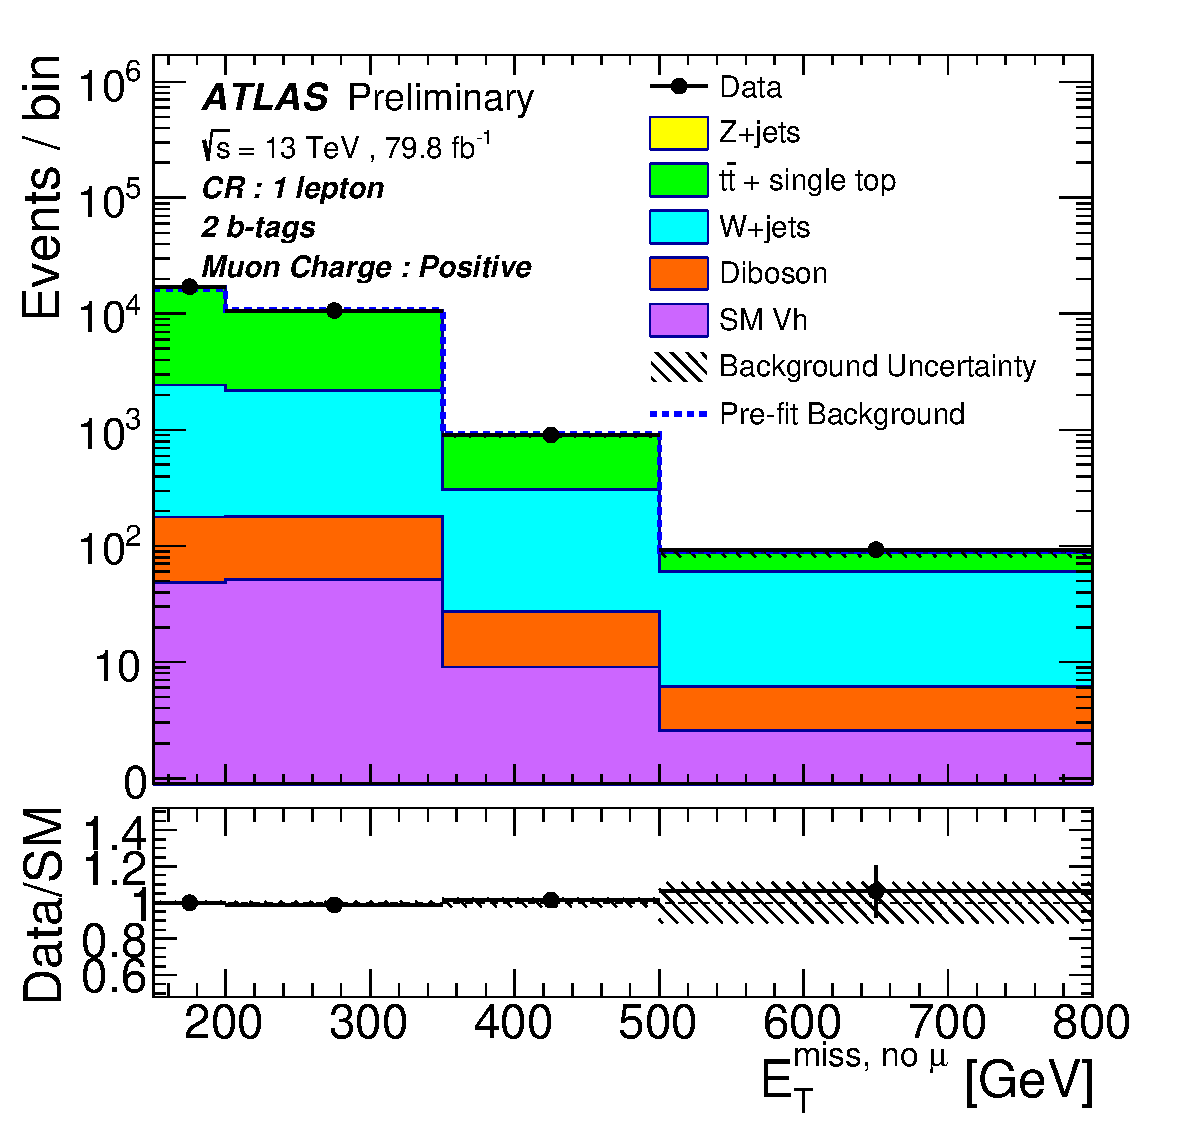
\includegraphics[width=.7\textwidth]{figures/monoH/results/fig_05a.pdf}
    \caption{1 muon CR \metnomu distribution (positive muon charge)}
  \end{subfigure}
  \\
  \begin{subfigure}{1.\textwidth}
    \centering
    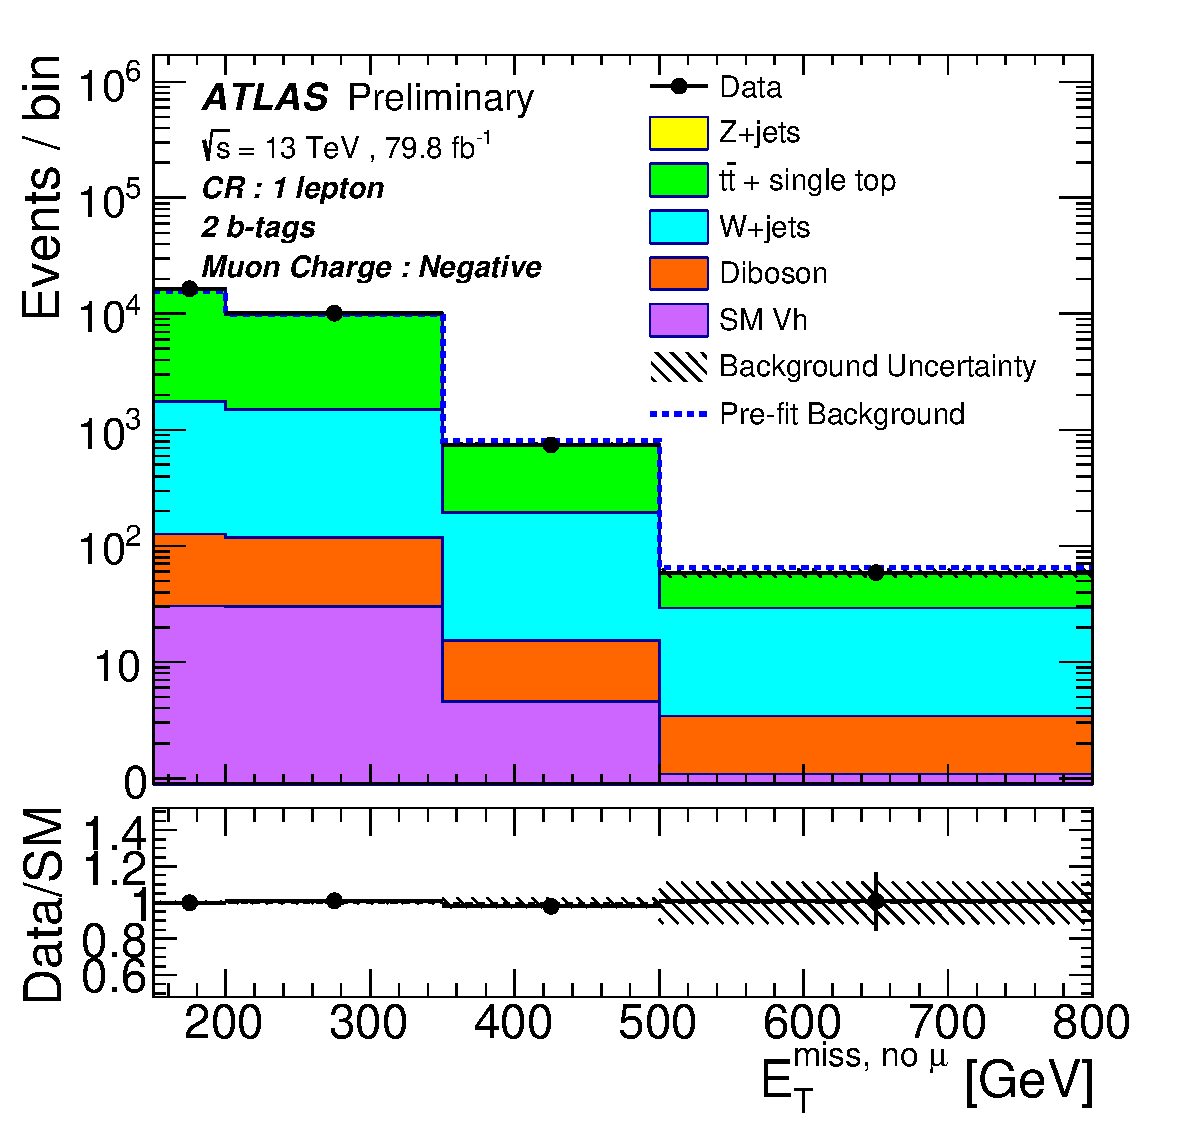
\includegraphics[width=.7\textwidth]{figures/monoH/results/fig_05b.pdf}
    \caption{1 muon CR \metnomu distribution (negative muon charge)}
  \end{subfigure}
  \caption{\metnomu distributions for the 1 muon CR, positive (top) and negative (bottom) muon charge shown separately. The upper panel shows the comparison of data to the SM background expectation before~(dashed lines) and after the background-only fit~(solid histograms). The lower panel shows the ratio of the data to SM background expectations after the background-only fit, with the hatched band showing the systematic uncertainty.}
  \label{fig:monoH:results:observed:cr1}
\end{figure}

\begin{figure}[htbp]
\centering
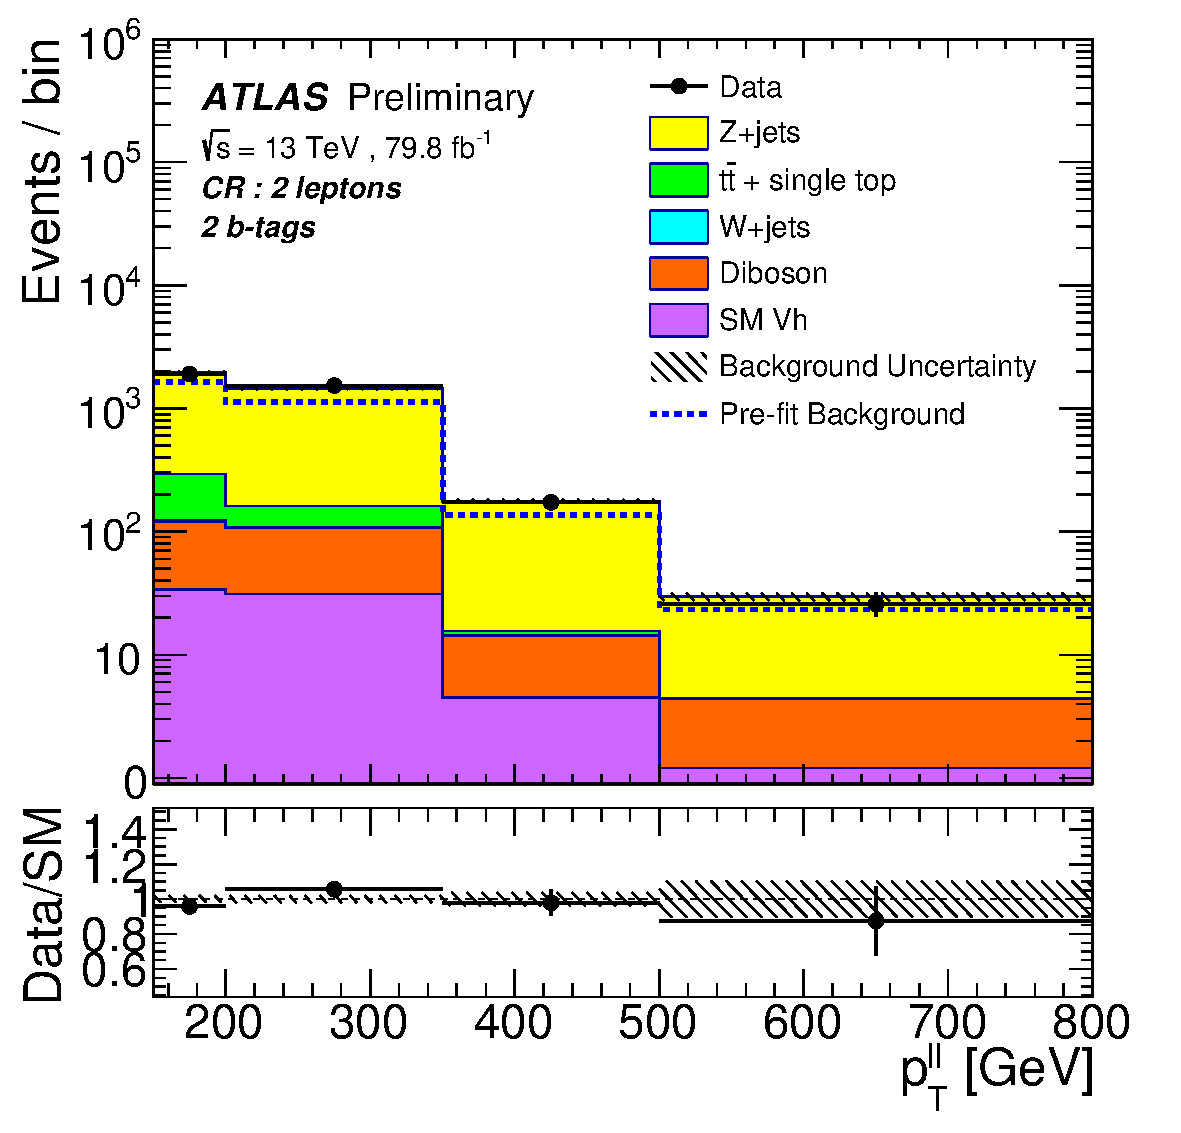
\includegraphics[width=0.95\textwidth]{figures/monoH/results/fig_05c.pdf}
\caption{\ptll distribution for the 2 lepton CR. The upper panel shows the comparison of data to the SM background expectation before~(dashed lines) and after the background-only fit~(solid histograms). The lower panel shows the ratio of the data to SM background expectations after the background-only fit, with the hatched band showing the systematic uncertainty.}
  \label{fig:monoH:results:observed:cr2}
\end{figure}


The results of the profile likelihood fit of the statistical model to the data are reported in terms of the discovery significance for \zhdm simplified model signals in dependence of \mZp and \mA in \Cref{fig:monoH:results:results:observed:significance}.

\begin{figure}[htbp]
\centering
  \begin{subfigure}{1.\textwidth}
    \centering
    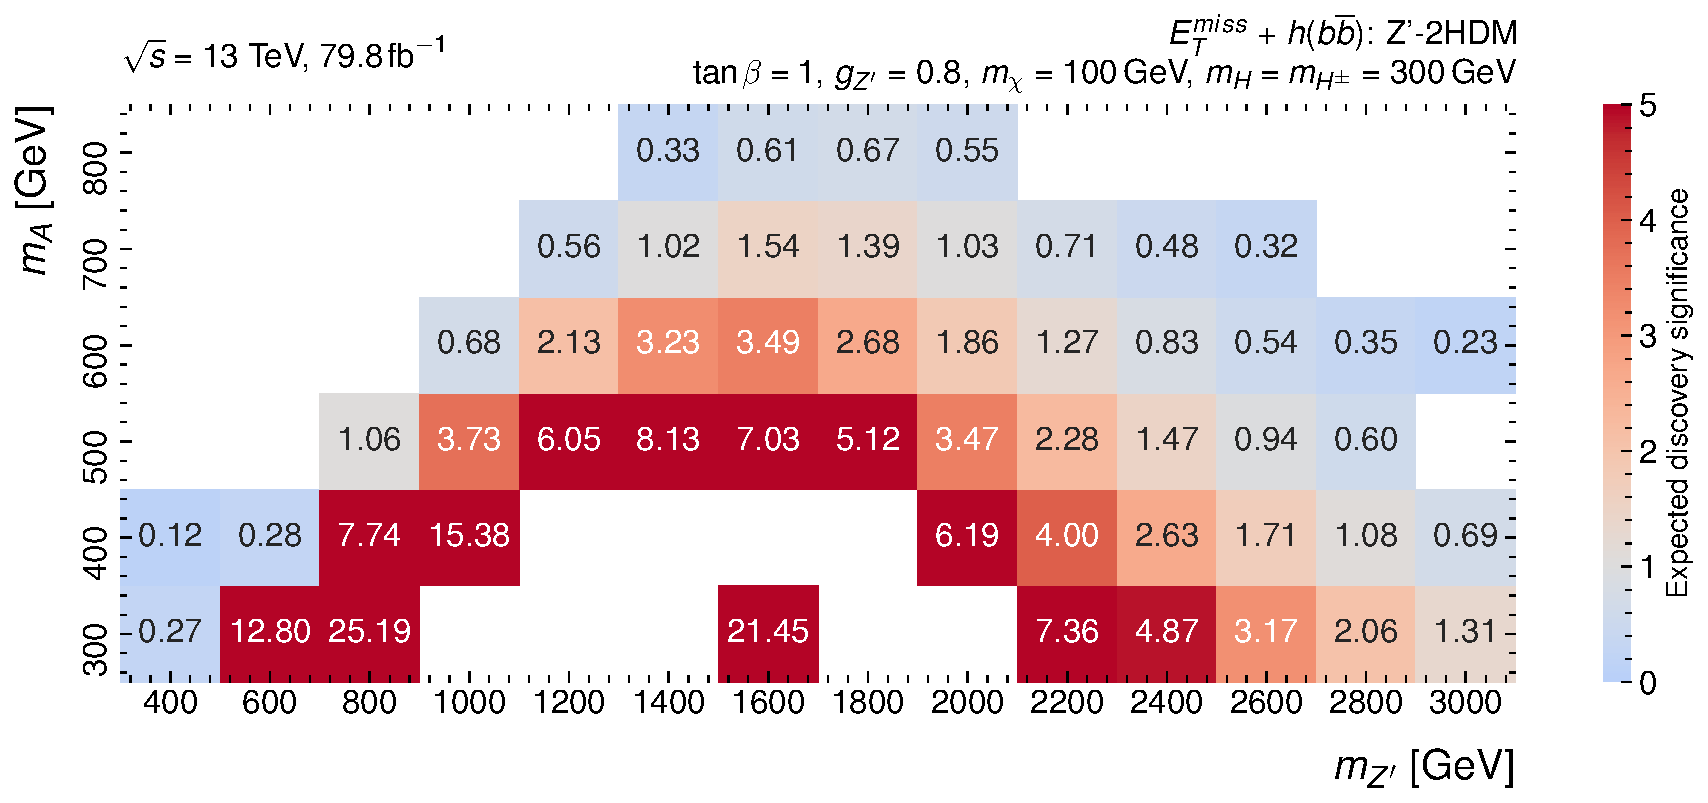
\includegraphics[width=0.95\textwidth]{figures/monoH/monoHbb-zhdm-significances_expected.pdf}
    \caption{Expected median discovery significance}
  \end{subfigure}
  \\
  \begin{subfigure}{1.\textwidth}
    \centering
    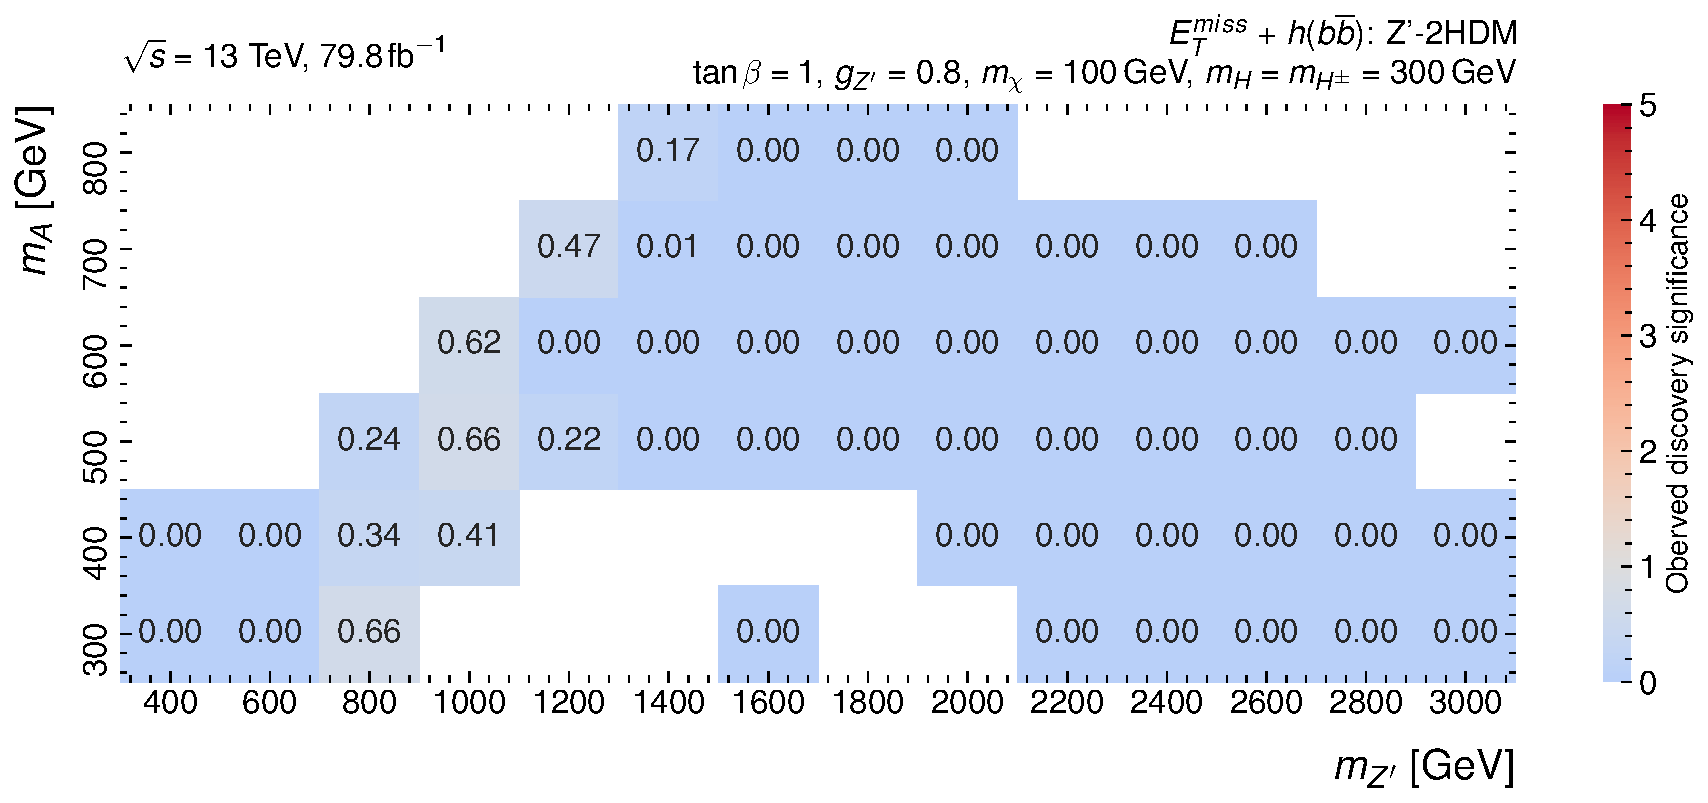
\includegraphics[width=0.95\textwidth]{figures/monoH/monoHbb-zhdm-significances_observed.pdf}
    \caption{Observed discovery significance}
  \end{subfigure}
  \caption{Expected median discovery significance \(Z^{\text{exp}}\)~(top) estimated with the Asimov dataset generated under the assumption of the nominal signal model (\(\mu=1\)) and observed discovery significance~(bottom) for the \zhdm simplified model signals in dependence of \PZprime mediator mass \mZp and CP-odd Higgs boson mass \mA.}
  \label{fig:monoH:results:results:observed:significance}
\end{figure}

No significant deviations from the background-only hypothesis have been observed. Therefore, the results in SR are presented with the background normalisations scaled to the outcome of the conditional background-only (\(\mu = 0\)) fit.

The observed number of events in the SR event selection for each \met bin is shown in \Cref{tab:monoH:results:observed:yield}. The expected number of events for the individual background processes, whose normalisation is determined by the background-only profile likelihood fit, and the observed events in data are shown.

\begin{table}[hbtp]
\caption{Expected and observed numbers of events in the signal region for an integrated luminosity of \SI{79.8}{\per\femto\barn} and \(\sqrt{s} = \SI{13}{\giga\electronvolt}\). The background yields and uncertainties are shown after the profile-likelihood fit to the data. The quoted background uncertainties include both the statistical and the systematic contributions.}
\label{tab:monoH:results:observed:yield}
\centering
\resizebox{1.\textwidth}{!}{%
\sisetup{round-mode=figures, round-precision=2,
         retain-explicit-plus=true, group-digits=integer, group-minimum-digits=4}
\begin{tabular}{l%
S[table-format=5.1, table-number-alignment=right, round-mode=figures, round-precision=3]@{$\,\pm\,$}
S[table-format=3.1, table-number-alignment=right, round-mode=figures, round-precision=2]@{\quad}
S[table-format=5.1, table-number-alignment=right, round-mode=figures, round-precision=3]@{$\,\pm\,$}
S[table-format=3.1, table-number-alignment=right, round-mode=figures, round-precision=2]@{\quad}
S[table-format=4.1, table-number-alignment=right, round-mode=figures, round-precision=3]@{$\,\pm\,$}
S[table-format=2.1, table-number-alignment=right, round-mode=figures, round-precision=2]@{\quad}
S[table-format=3.2, table-number-alignment=right, round-mode=figures, round-precision=3]@{$\,\pm\,$}
S[table-format=2.2, table-number-alignment=right, round-mode=figures, round-precision=2]@{\quad}}
\toprule
\multirow{2}{*}{Process} & \multicolumn{8}{c}{Range in \met [\si{\giga\electronvolt}]} \\
& \multicolumn{2}{c}{\([150,200)\)} & \multicolumn{2}{c}{\([200,350)\)} & \multicolumn{2}{c}{\([350,500)\)} & \multicolumn{2}{c}{\([500,\infty)\)}\\
\midrule
\ttbar + single top quark & 11796.86 & 349.61 & 6450.18 & 197.21 & 307.6 & 24.91 & 10.8 & 2.52 \\
\wjets & 3023.56 & 529.59 & 2237.96 & 359.05 & 183.63 & 31.85 & 26.38 & 5.67 \\
\zjets & 6333.38 & 453.25 & 5176.41 & 343.31 & 564.95 & 37.21 & 80.51 & 6.32 \\
Diboson & 438.35 & 67.15 & 399.62 & 59.17 & 48.98 & 11.2 & 9.37 & 1.72 \\
\VHbb & 136.33 & 38.83 & 129.3 & 36.91 & 17.26 & 4.95 & 3.86 & 1.12 \\
\midrule
Background & 21728.48 & 137.51 & 14393.46 & 110.23 & 1122.44 & 25.27 & 130.92 & 7.16 \\
Data &  \multicolumn{2}{l}{\dat{21818.0}}   &  \multicolumn{2}{@{}l}{\dat{14350.0}} & \multicolumn{2}{@{}l}{\dat{1128.0}} & \multicolumn{2}{@{}l}{\dat{119.0}} \\
\bottomrule
\end{tabular}%
}
\end{table}

The corresponding \met distribution is shown in \Cref{fig:monoH:results:observed:met}. No significant excess over the SM background is observed.

\begin{figure}[htbp]
\centering
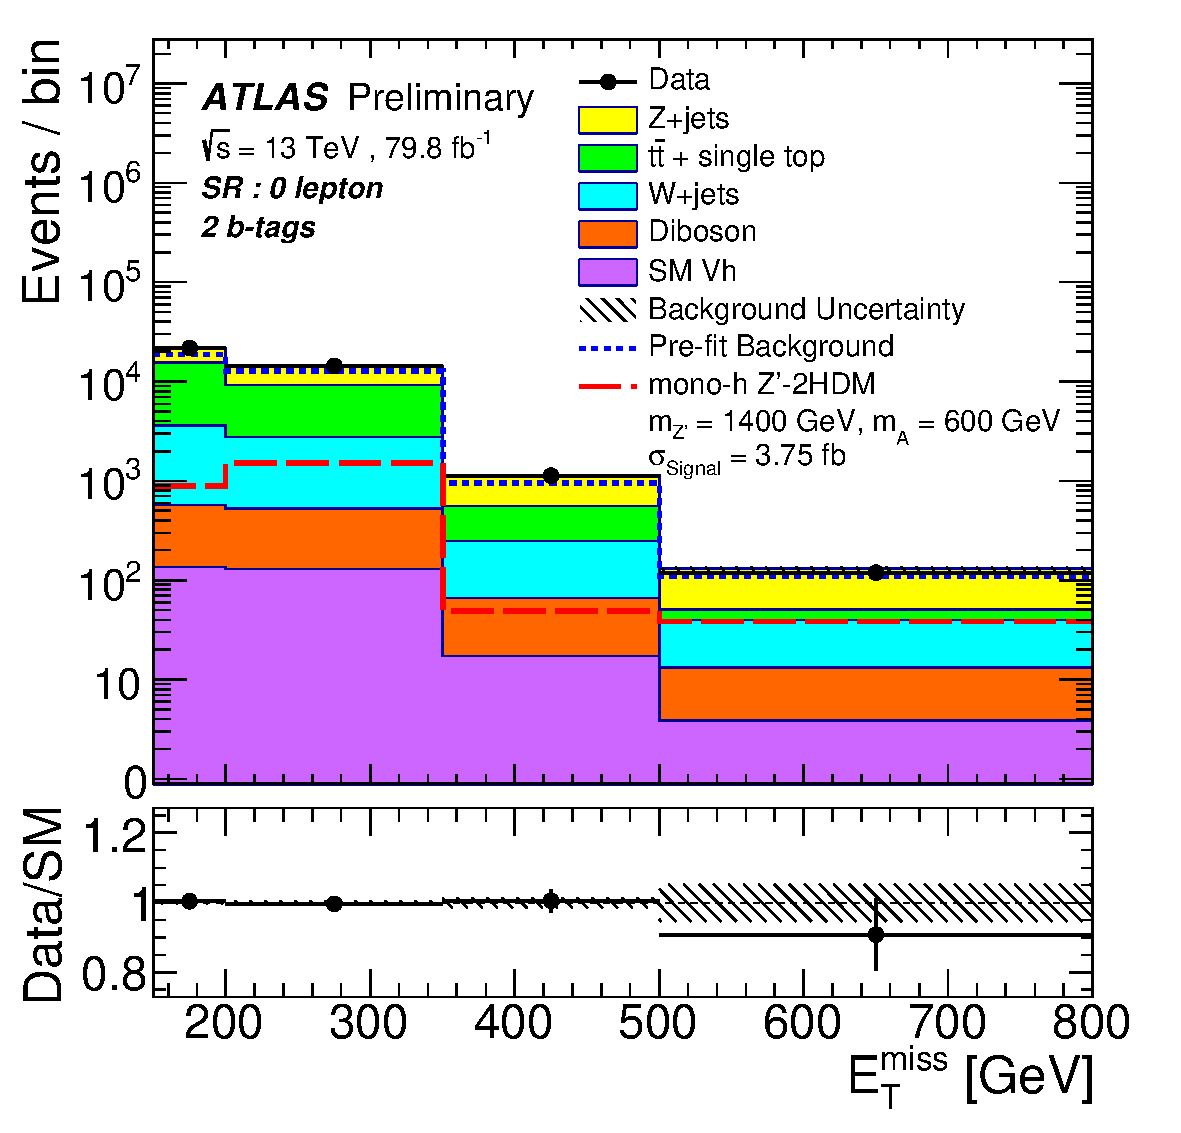
\includegraphics[width=0.95\textwidth]{figures/monoH/results/fig_07.pdf}
\caption{\met distribution for the SR. The upper panel shows the comparison of data to the SM background expectation before~(dashed lines) and after the background-only fit~(solid histograms). The expected distribution for a representative \zhdm signal is overlaid~(long-dashed line). The lower panel shows the ratio of the data to SM background expectations after the background-only fit, with the hatched band showing the systematic uncertainty.}
  \label{fig:monoH:results:observed:met}
\end{figure}

The invariant mass distributions in the SR are shown in \Cref{fig:monoH:results:observed:mass}. The signal process is characterised by a large Higgs boson mass peak, which is most evident in the merged category due to the relatively low contribution of background processes.

\begin{figure}[htbp]
\centering
  \begin{subfigure}{0.45\textwidth}
    \centering
    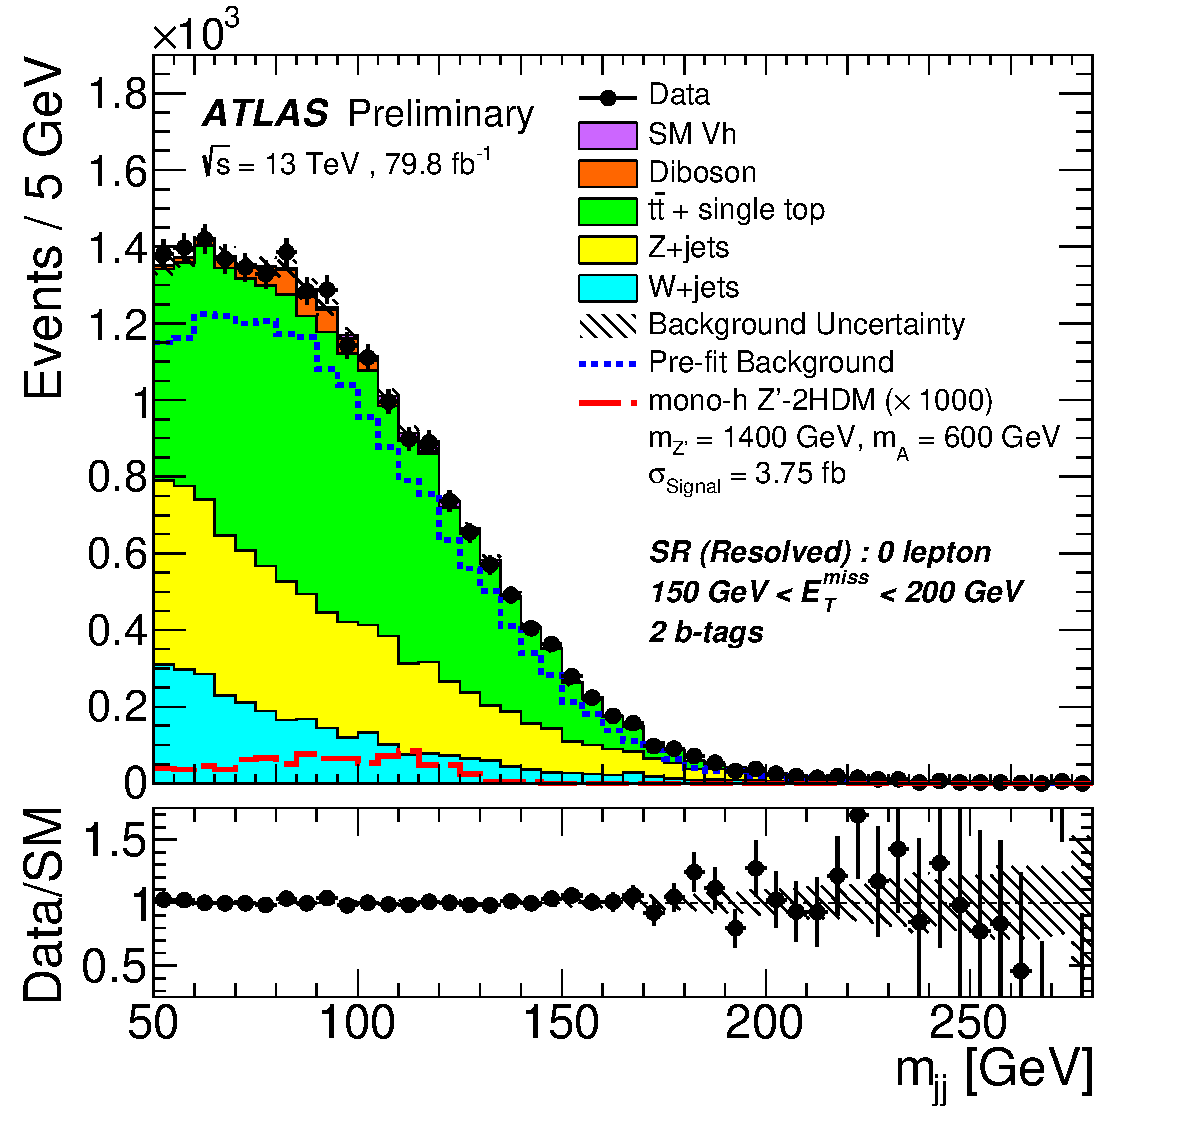
\includegraphics[width=0.95\textwidth]{figures/monoH/results/fig_06a.pdf}
    \caption{SR resolved category \\\(\SI{150}{\giga\electronvolt} < \met < \SI{200}{\giga\electronvolt}\)}
  \end{subfigure}
  \begin{subfigure}{0.45\textwidth}
    \centering
    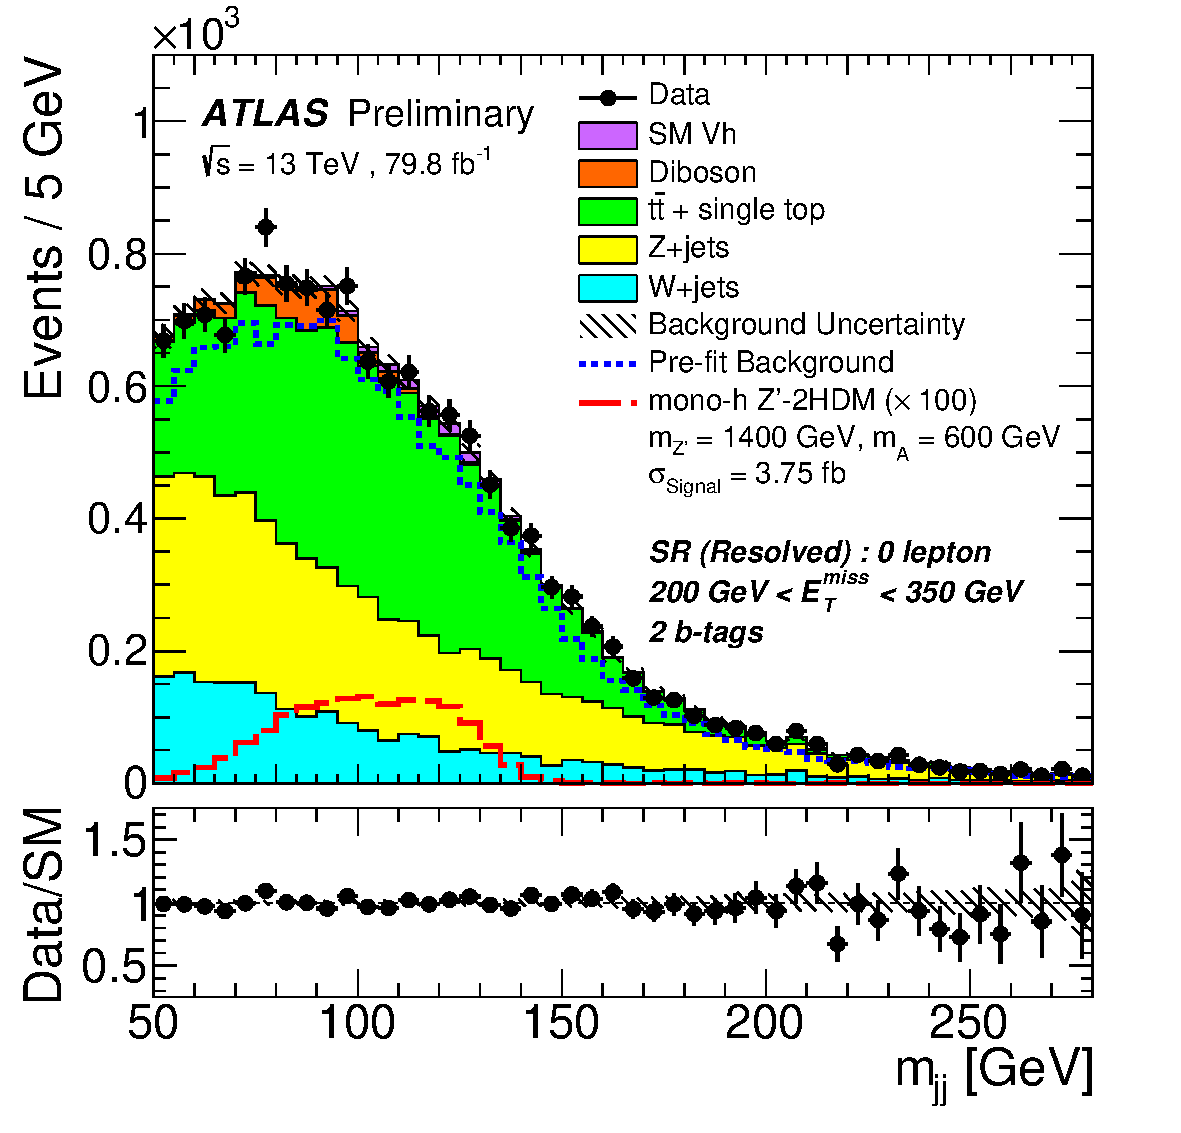
\includegraphics[width=0.95\textwidth]{figures/monoH/results/fig_06b.pdf}
    \caption{SR resolved category \\\(\SI{200}{\giga\electronvolt} < \met < \SI{350}{\giga\electronvolt}\)}
  \end{subfigure}
  \\
  \begin{subfigure}{0.45\textwidth}
    \centering
    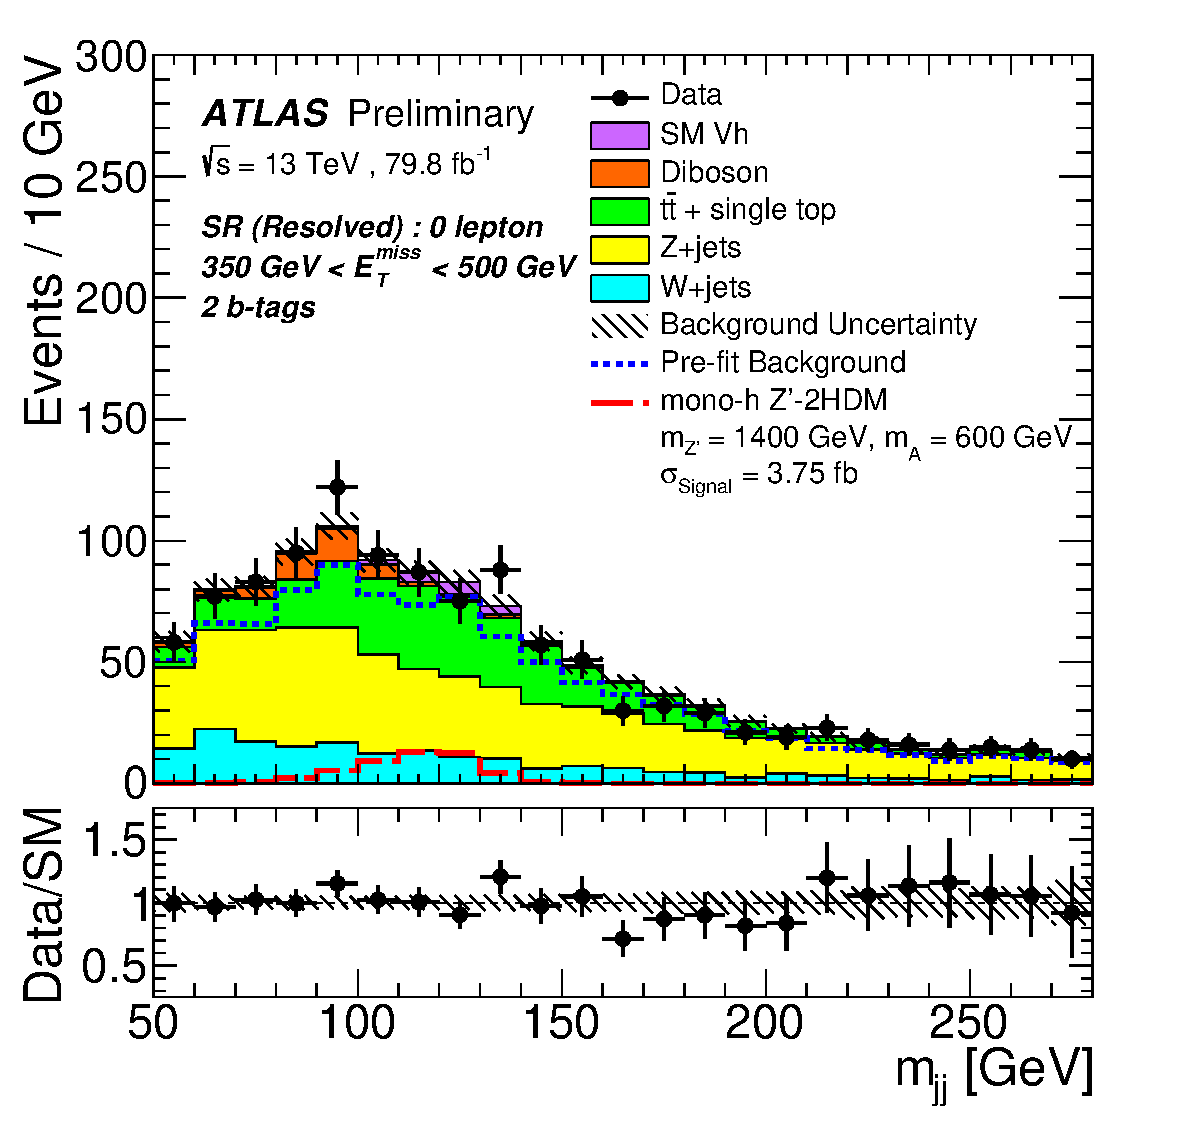
\includegraphics[width=0.95\textwidth]{figures/monoH/results/fig_06c.pdf}
    \caption{SR resolved category \\\(\SI{350}{\giga\electronvolt} < \met < \SI{500}{\giga\electronvolt}\)}
  \end{subfigure}
  \begin{subfigure}{0.45\textwidth}
    \centering
    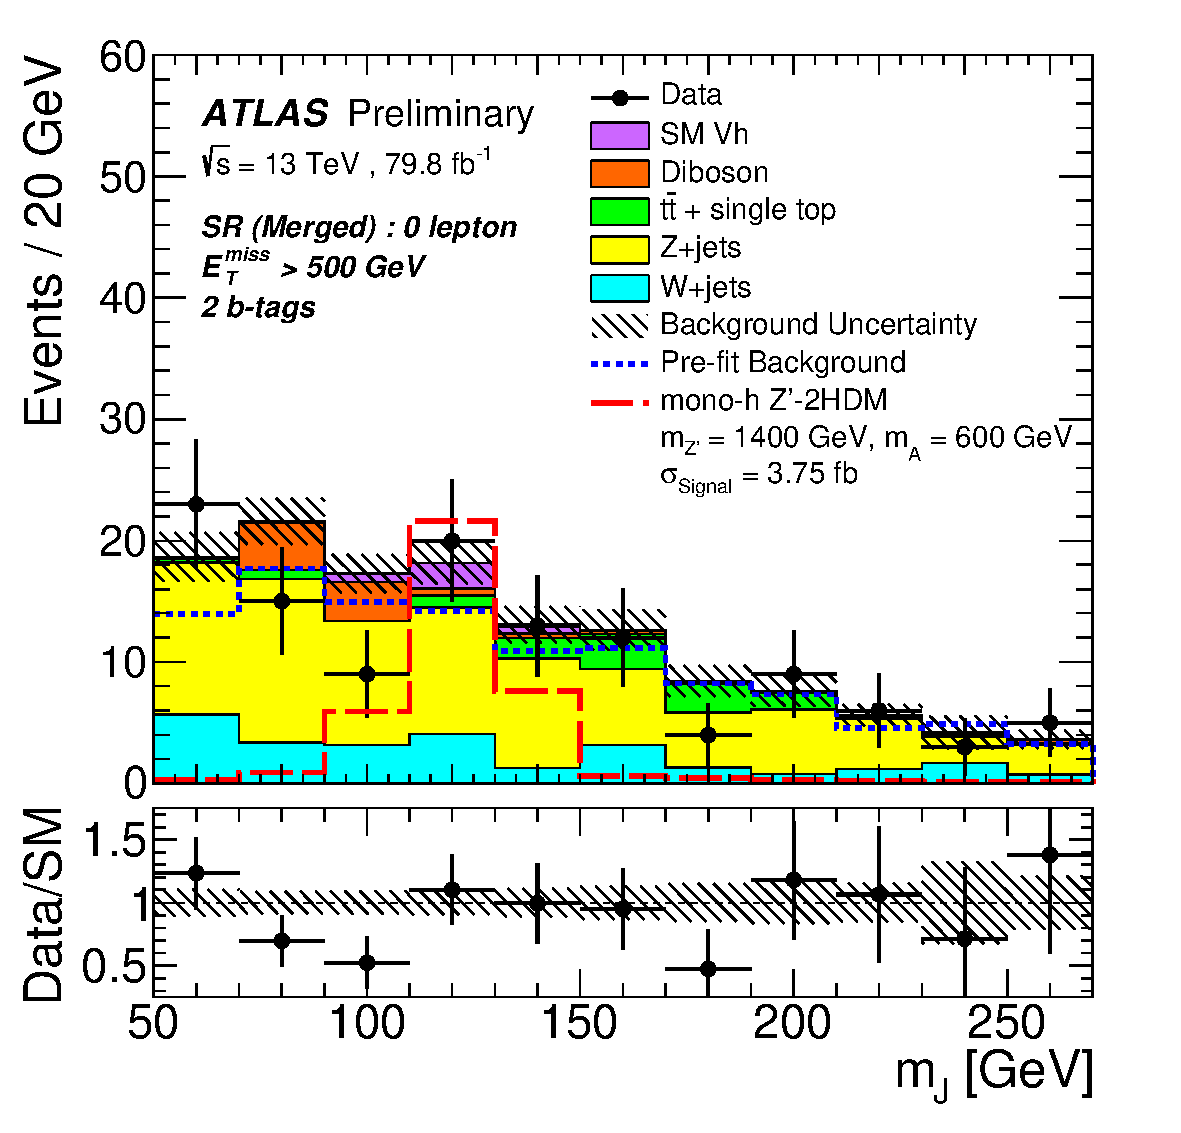
\includegraphics[width=0.95\textwidth]{figures/monoH/results/fig_06d.pdf}
    \caption{SR merged category \\ \(\met > \SI{500}{\giga\electronvolt}\)}
  \end{subfigure}
  \caption{Distributions of the Higgs boson candidate invariant mass \(m_{jj}\) (resolved) and \(m_{J}\) (merged) in the SR for the four \met bins. The upper panels show a comparison of data to the SM expectation before~(dashed lines) and after the background-only fit~(solid histograms). The expected distribution for a representative \zhdm signal is overlaid~(long-dashed line) and scaled by factors of \num{1000} and \num{100} in the two lowest \met bins. The lower panels show the ratio of the data to SM background expectations after the background-only fit, with the hatched band indicating the systematic uncertainty.}
  \label{fig:monoH:results:observed:mass}
\end{figure}


\subsection{Impact of systematic uncertainties}
\label{sec:monoH:results:impact}
The impact of the various sources of systematic uncertainty on the fitted signal strength \(\mu\) is evaluated using the procedure presented in \Cref{sec:monoV:results:impact}.

\Cref{tab:monoH:results:impact:breakdown} shows a breakdown of the expected signal strength uncertainties for three representative \zhdm simplified model signals. The first signal corresponds to events selected primarily in the resolved category. The second signal corresponds to equal contributions of the merged and resolved categories. The third signal corresponds to events selected primarily in the merged category.
The dominant sources of uncertainty are due to the identification of \btagged jets, modelling uncertainties in \ttbar and \vjets processes, and statistical uncertainty in the background prediction.
The impact of large-radius jet uncertainties and the statistical uncertainty in the background prediction increases for the second and third signals because of a larger fraction of events in the merged category.
For signals with heavy \mZp, the total uncertainty is dominated by the statistical uncertainty of data.

\begin{table}[hbtp]
  \caption{Breakdown of expected signal strength uncertainties for three representative \zhdm signal samples (a)~\((\mZp, \mA) = (\SI{0.6}{\tera\electronvolt},\SI{0.3}{\tera\electronvolt})\), (b)~\((\mZp, \mA) = (\SI{1.4}{\tera\electronvolt},\SI{0.6}{\tera\electronvolt})\), and (c)~\((\mZp, \mA) = (\SI{2.6}{\tera\electronvolt},\SI{0.3}{\tera\electronvolt})\). The effect is expressed as the relative uncertainty on the signal strength, assuming total cross-sections of (a)~\SI{452}{\femto\barn}, (b)~\SI{3.75}{\femto\barn}, and (c)~\SI{2.03}{\femto\barn}. Each systematic uncertainty contribution is provided as the quadratic difference between the total uncertainty and the uncertainty obtained by setting the systematic uncertainty in question to its nominal value and excluding it thereby from the fit. Total denotes the quadrature sum of statistical and total systematic uncertainties.}
  \label{tab:monoH:results:impact:breakdown}
  \centering
  \begin{tabular}{l rrr}
  \toprule
  Source & \multicolumn{3}{c}{Uncertainty on \(\mu\) [\si{\percent}]} \\
  of uncertainty & (a) & (b) & (c) \\
  \midrule
  \btagging             & 4.0  & 8.0   & 10\phdo \\
  Large-radius jets     & 0.2  & 1.0   & 2.0     \\
  Small-radius jets     & 1.4  & 3.0   & 2.0     \\
  \met                  & 1.2  & 1.7   & 1.1     \\
  Leptons               & 0.2  & 0.8   & 0.7     \\
  Luminosity            & 2.0  & 2.5   & 2.5     \\
  & & & \\
  Signal modelling      & 3.0  & 2.5   & 1.5     \\
  Top quark modelling   & 3.7  & 4.8   & 4.5     \\
  \vjets modelling      & 3.5  & 6.0   & 5.0     \\
  SM \VHbb modelling    & 0.8  & 3.2   & 2.1     \\
  Diboson modelling     & 0.8  & 1.5   & 1.1     \\
  Background MC stat.   & 1.8  & 5.4   & 4.9     \\
  \midrule
  Total syst.           & 6.5    & 13\phdo  & 13\phdo \\
  Data stat.            & 2.3    & 20\phdo  & 22\phdo \\
  Total                 & 7\phdo & 24\phdo  & 25\phdo \\
  \bottomrule
  \end{tabular}
\end{table}


\subsection{Constraints on the \zhdm simplified model}
\label{sec:monoH:results:limits-zhdm}
As no significant deviation from the SM background expectation is observed for any of the signal mass points, the  parameter space of the \zhdm simplified model can be constrained by computing upper limits on the signal strength \(\mu\) at \SI{95}{\percent} confidence level using the \(\text{CL}_{s}\) method~\cite{Read:2002hq}.

The exclusion limit contour, which is provided in the two-dimensional \mZp-\mA plane for the fixed set of parameters  \(g_{\PZprime} = 0.8\), \(\tan \beta = 1\), \(\mchi = \SI{100}{\giga\electronvolt}\), and \(\mHiggsHeavy = \mHiggsCharged = \SI{300}{\giga\electronvolt}\), is shown in \Cref{tab:monoH:results:limits-zhdm:contour}.
The signal points in the \zhdm model with \mZp of up to \SI{2.85}{\tera\electronvolt} and \mA up to \SI{670}{\giga\electronvolt} are excluded at \SI{95}{\percent} \(\text{CL}_{s}\), slightly exceeding the expected exclusion of the \PZprime masses of up to \SI{2.7}{\tera\electronvolt}.

\begin{figure}[htbp]
    \centering
    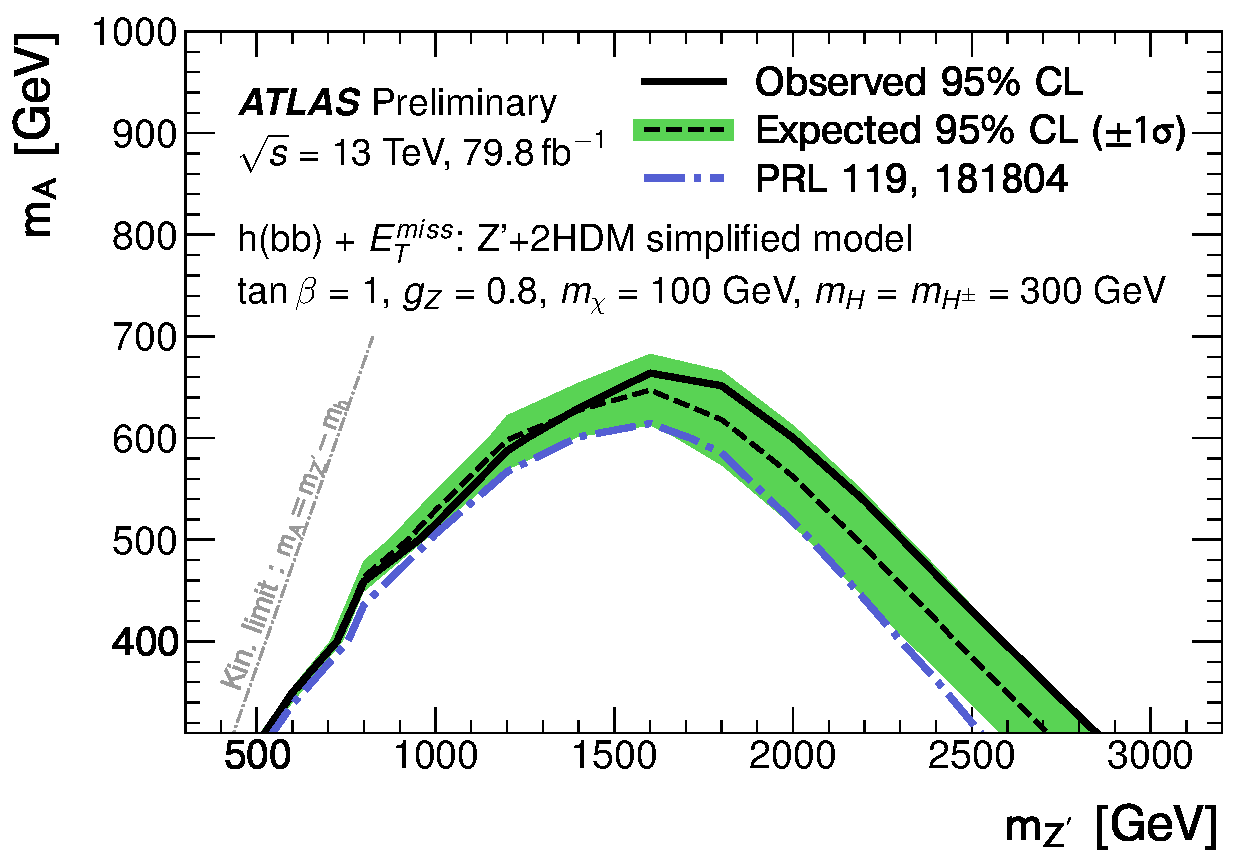
\includegraphics[width=.95\textwidth]{figures/monoH/results/fig_08.pdf}
    \caption{Exclusion contours at \SI{95}{\percent} \(\text{CL}_{s}\) for the \zhdm simplified model in the \mZp-\mA plane for the fixed set of parameters \(\tan{\beta} = 1.0\), \(g_{\PZprime} = 0.8\), and \(\mchi = \SI{100}{\giga\electronvolt}\). The observed limits~(solid line) are consistent with the expectation under the SM-only hypothesis~(densely dashed line) within uncertainties~(filled band). The observed exclusion contour from a previous ATLAS publication at \(\sqrt{s} = \SI{13}{\tera\electronvolt}\)~(dash-dotted line)~\cite{EXOT-2016-25} is overlaid.}
    \label{tab:monoH:results:limits-zhdm:contour}
\end{figure}

The improvement from using VR track jets instead of FR track jets is demonstrated in \Cref{tab:monoH:results:limits-zhdm:limit}. The expected upper limits on the signal strength \(\mu\) obtained with VR track jets is compared against that of the search presented in Ref.~\cite{EXOT-2016-25}, which is obtained using fixed-radius (FR) track jets. The latter is scaled to \SI{79.8}{\femto\barn} and computed by only considering events with two \bjets. Other differences between the two searches include the suppression of the multijet background using the object-based \met significance, reduced statistical uncertainties from the MC background simulation, and an improved \btagging calibration for VR track jets. The expected limits for \zhdm signals with highly boosted Higgs bosons show a significant improvement of up to a factor of three. Thus, this search based on VR track jets outperforms its predecessor considerably.

\begin{figure}[htbp]
    \centering
    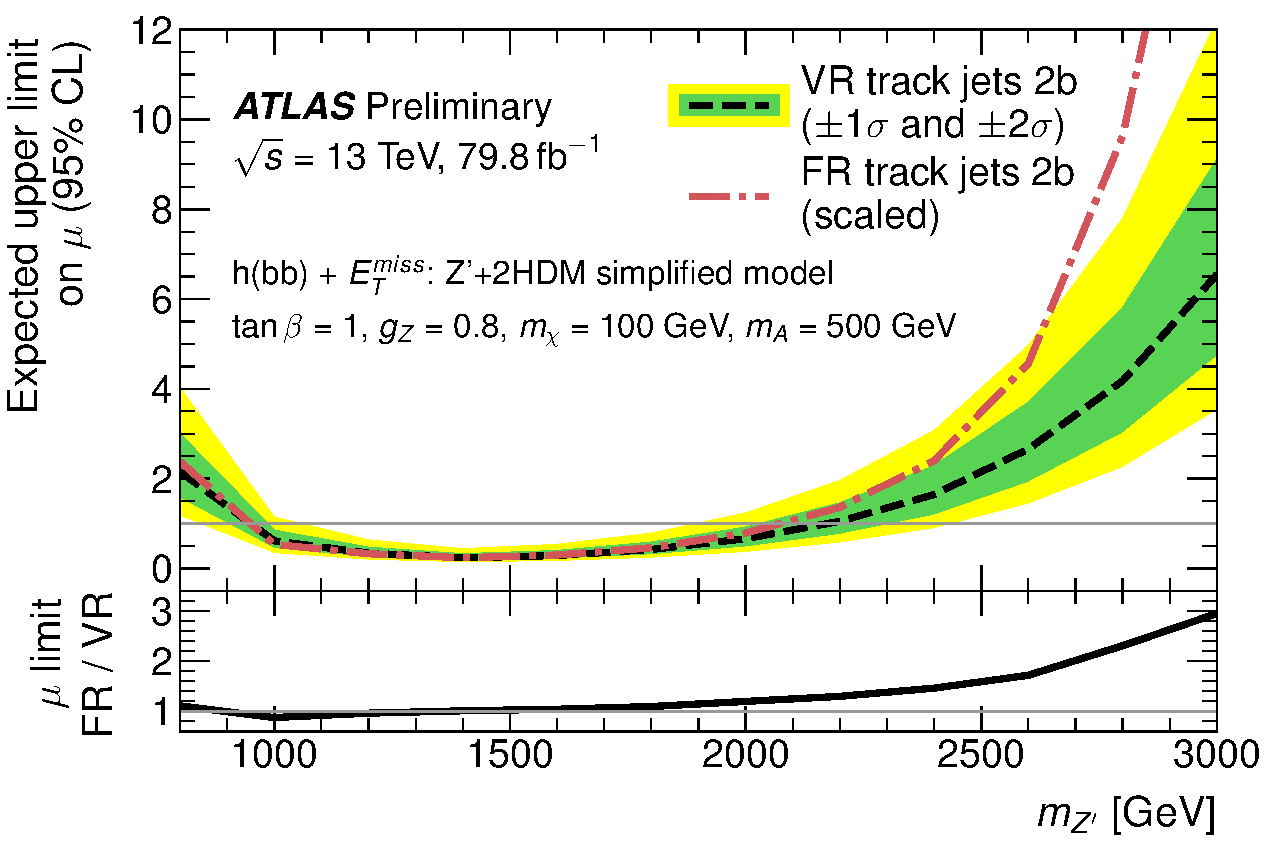
\includegraphics[width=.95\textwidth]{figures/monoH/results/fig_09.pdf}
    \caption{Expected exclusion limit on the signal strength \(\mu\) at \SI{95}{\percent} \(\text{CL}_{s}\) in dependence of \mZp for the \zhdm simplified model for the fixed set of parameters \(\mA = \SI{500}{\giga\electronvolt}\), \(\tan{\beta} = 1.0\), \(g_{\PZprime} = 0.8\), and \(\mchi = \SI{100}{\giga\electronvolt}\). %
    The expected limit of this search~(dashed line) using variable-radius (VR) track jets is compared against that of the search presented in Ref.~\cite{EXOT-2016-25} using fixed-radius (FR) track jets. The latter is scaled to \SI{79.8}{\femto\barn} and computed by only considering events with two \bjets. Other differences between the two searches include the suppression of the multijet background using the object-based \met significance, reduced statistical uncertainties from the MC background simulation, and an improved \btagging calibration for VR track jets. %
    The lower panel shows the ratio of the expected limit obtained with VR track jets and FR track jets.}
    \label{tab:monoH:results:limits-zhdm:limit}
\end{figure}

\section{Conclusion of the \(\met + \Hbb\) search}
\label{sec:monoH:conclusion}
In conclusion, the novelty of VR track jets is applied in this search, and its superior performance in events with highly boosted Higgs candidates is established.
The null results push the viable parameter space for yet unobserved resonances to yet higher masses, thereby increasing the relevance of event topologies with highly boosted objects.
The VR track jet technique enables searches targeting these event topologies and is eagerly adopted by the experimental community~\cite{ATLAS-CONF-2018-052,EXOT-2018-48,HIGG-2018-52,ATLAS-CONF-2020-043}.
